\documentclass{article}


\usepackage{PRIMEarxiv}

\usepackage[utf8]{inputenc} % allow utf-8 input
\usepackage[T1]{fontenc}    % use 8-bit T1 fonts
\usepackage{hyperref}       % hyperlinks
\usepackage{url}            % simple URL typesetting
\usepackage{booktabs}       % professional-quality tables
\usepackage{amsfonts}       % blackboard math symbols
\usepackage{nicefrac}       % compact symbols for 1/2, etc.
\usepackage{microtype}      % microtypography
\usepackage{lipsum}
\usepackage{fancyhdr}       % header
\usepackage{graphicx}       % graphics
\graphicspath{{media/}}     % organize your images and other figures under media/ folder
\usepackage{booktabs}
\usepackage{amsmath}
\usepackage{graphicx}
\usepackage{subcaption}
\usepackage[utf8]{inputenc}
\usepackage[ruled,longend]{algorithm2e}
\usepackage{textgreek}
\usepackage{amssymb}
\usepackage{graphicx}
\usepackage{subcaption}
\usepackage{diagbox}
\usepackage{multirow}
%Header
\pagestyle{fancy}
\thispagestyle{empty}
\rhead{ \textit{}} 



  
%% Title
\title{Continual Scene Detection}

\author{
  Leon Li \\
  Columbia University \\
  New York\\
  \texttt{\{al4263\}@columbia.edu} \\
  %% examples of more authors
  %% \AND
  %% Coauthor \\
  %% Affiliation \\
  %% Address \\
  %% \texttt{email} \\
  %% \And
  %% Coauthor \\
  %% Affiliation \\
  %% Address \\
  %% \texttt{email} \\
  %% \And
  %% Coauthor \\
  %% Affiliation \\
  %% Address \\
  %% \texttt{email} \\
}


\begin{document}
\maketitle


\begin{abstract}
In this paper, we propose a novel method for training fluid queues using direct backpropagation, capitalizing on their differentiable dynamics compared to traditional stochastic queueing networks. Fluid queues, which disregard the inherent stochasticity in arrival and service processes, offer a fully deterministic framework for modeling and optimization. By employing modern deep neural network architectures and leveraging the continuous nature of fluid queues, we can efficiently train a parametrized policy to minimize the cost of the system.
\end{abstract}


% keywords can be removed


\section{Problem Formulating}

In this paper, we investigate the problem of continual scene detection. A \textit{frame} $\boldsymbol{f}$ is defined as a vector $\mathbb{R}^n$ where each component is sampled from a Bernoulli distribution with probability $p=0.5$ with possible outcomes in the set $\{-1, 1\}$. A \textit{scene} $s$ is composed of $n=4$ frames. The first frame $\boldsymbol{f_1}$ being randomly generated and the subsequent frames being derived from the first frame with a degree of variation of $0.1$. Specifically, this means we randomly flip the values of $10\%$ of the components of $\boldsymbol{f_1}$ to create the subsequent frames. We continuously generate a stream of scenes. At a certain time point $t=R$, a decision is made to either generate a new scene or re-use the previous one to create a \textit{familiar scene}. If a familiar scene is chosen, the scene from time $t=T-R$ is permuted randomly. However, if a familiar scene is generated at time $t=T$, it will not be generated again at $t=T+R$. The task at hand is to continuously identify whether a presented scene is familiar or novel.


\section{Introduction to Memory Networks}

Memory Networks comprise of different architectural designs, which include a Memory Layer acting as the initial hidden layer, and a variety of types of readout layers. 

\subsection{Memory Layer}
The Memory Layer is a fully connected layer, endowed with either additive plasticity ($A$) or multiplicative plasticity ($M$). The weights and plasticity matrix at time $t$ for this layer are represented by $W_1$ and $P_1(t)$ respectively.

The method of updating the hidden layer hinges on the type of plasticity as described below:

\begin{itemize}
    \item \textbf{Multiplicative Plasticity (\textbf{M}):} The hidden layer $h_1(t)$ at time $t$ is updated using the following equation:
    \begin{equation}
    \boldsymbol{h_1}(t)=\phi\left(\left(\boldsymbol{W_1} \cdot \boldsymbol{P_1}(t)\right) \boldsymbol{x}(t)+\boldsymbol{W_1} \boldsymbol{x}(t)+\boldsymbol{b_1}\right)
    \end{equation}
    
    \item \textbf{Additive Plasticity (\textbf{A}):} The hidden layer $h_1(t)$ at time $t$ is updated as follows:
    \begin{equation}
    \boldsymbol{h_1}(t)=\phi\left(\left(\boldsymbol{W_1}+\boldsymbol{P_1}(t)\right) \boldsymbol{x}(t)+\boldsymbol{b_1}\right)
    \end{equation}
    
     \item \textbf{Stacked Plasticity (\textbf{Stack}):} The hidden layer $h_1(t)$ at time $t$ is for the Stacked Plasticity is generated by stacking a \textbf{M} and a \textbf{A}. So the upper half of the network works as the \textbf{M} and the second half works as \textbf{A}.
\end{itemize}

In these equations, $\phi$ represents the $\tanh$ function. The plasticity matrix update rule is expressed as follows for both types:

\begin{equation}
\boldsymbol{P}(t)=\lambda \boldsymbol{P}(t-1)+ \boldsymbol{\eta} \odot\left(\boldsymbol{h_1}(t) \boldsymbol{x}(t)^T\right)
\end{equation}

Observe that in this context, $\boldsymbol{\eta}$ is not a scalar. In fact, there exist three distinct forms of $\eta$, namely scalar, neuron-wise, and synaptic-wise. For scalar $\eta$, it retains its usual scalar nature. In the case of neuron-wise $\boldsymbol{\eta}$, it manifests as a vector of the same dimensions as $h_1(t)$, where each constituent of $\eta$ individually controls each row of $\boldsymbol{h_1}(t) \boldsymbol{x}(t)^T$. The synaptic-wise $\boldsymbol{\eta}$ form is a matrix identical in size to $\boldsymbol{h_1}(t) \boldsymbol{x}(t)^T$, with each element acting as a heterogenous learning rate for its corresponding element in $\boldsymbol{h_1}(t) \boldsymbol{x}(t)^T$.


\subsection{Readout Layer}

\begin{figure}[h!]
    \centering
    \begin{subfigure}{0.45\textwidth}
        \centering
        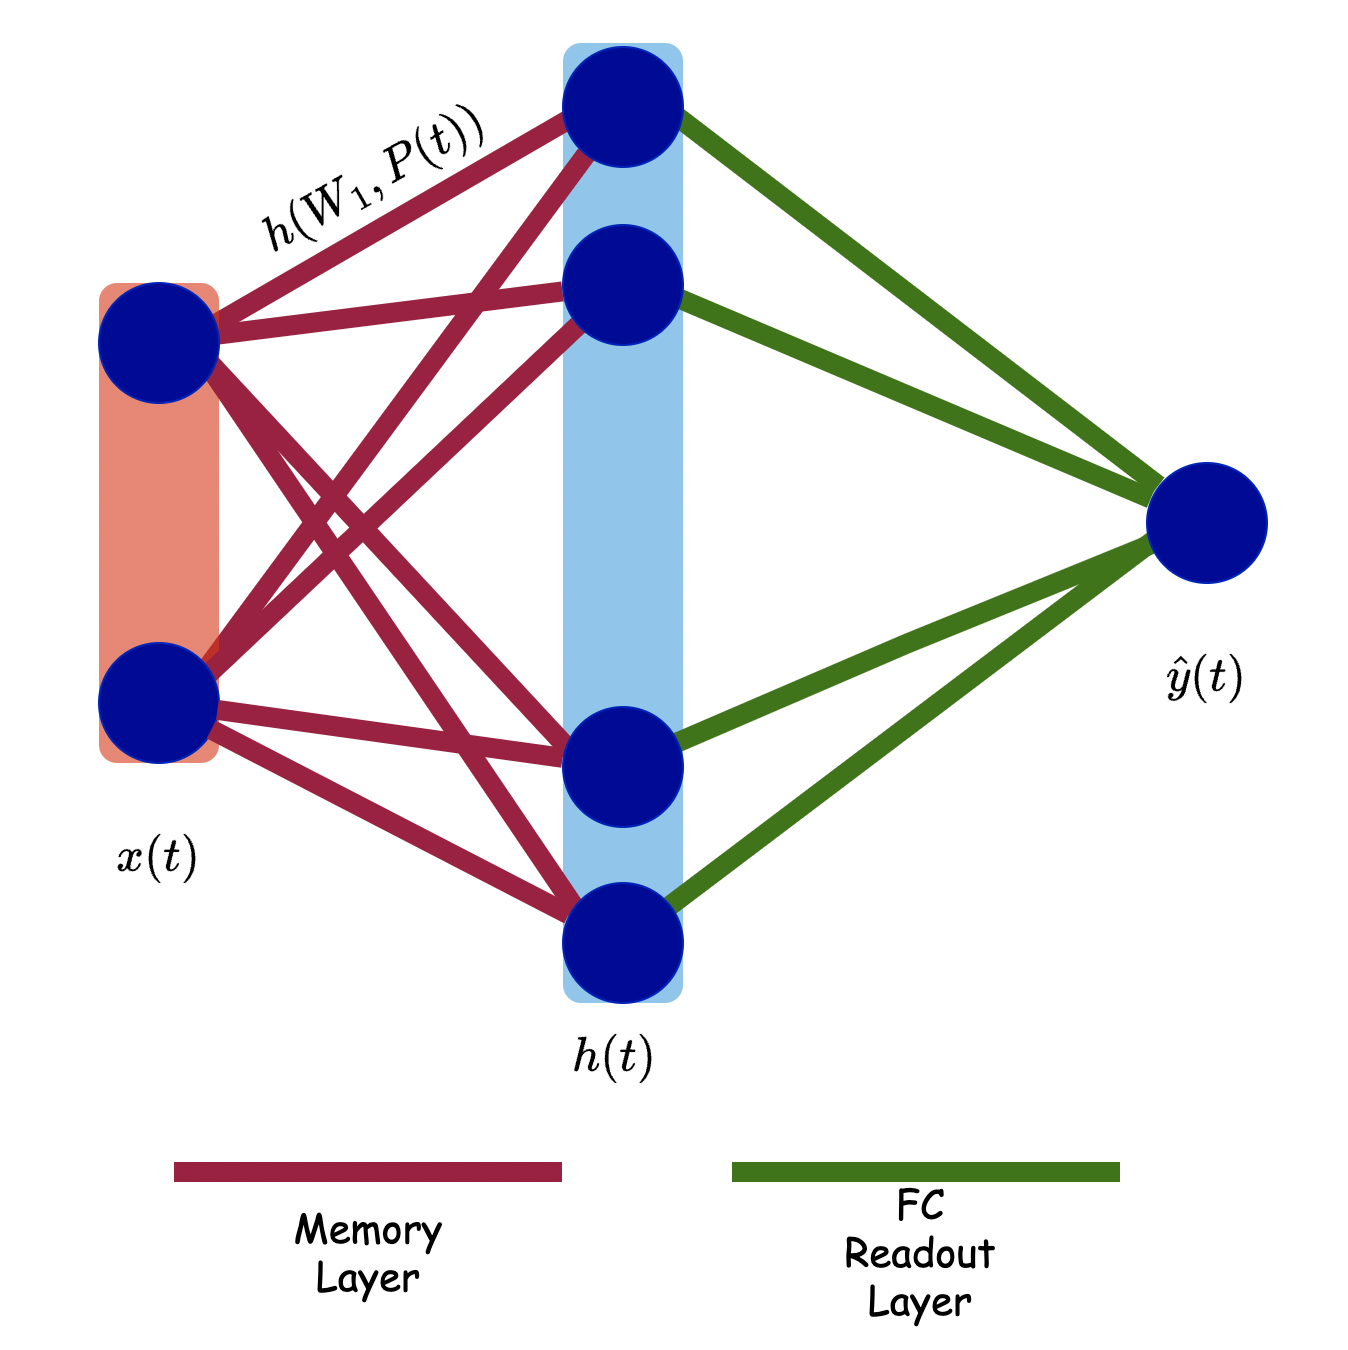
\includegraphics[width=\textwidth]{FC}
        \caption{Fully Connected Readout}
        \label{fig:fc}
    \end{subfigure}
    \hfill
    \begin{subfigure}{0.45\textwidth}
        \centering
        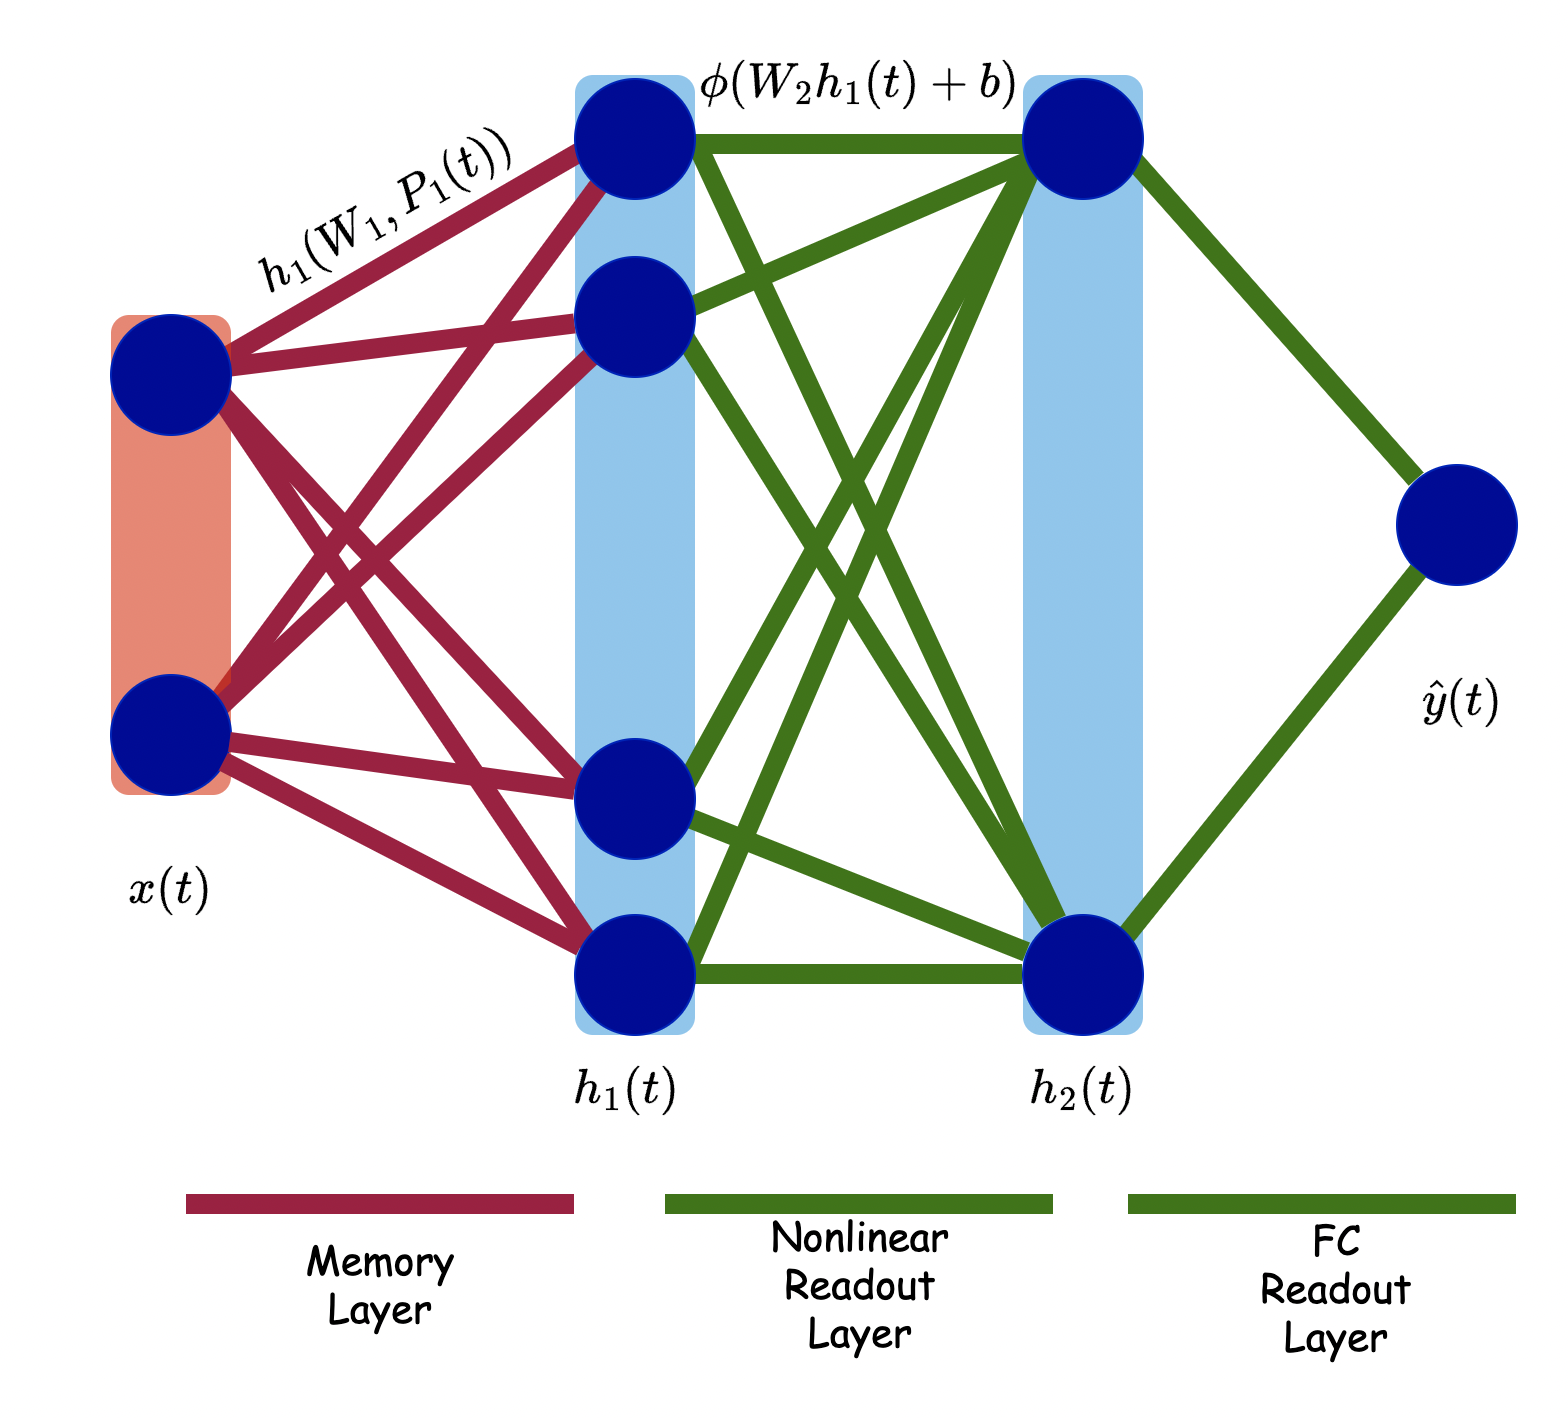
\includegraphics[width=\textwidth]{Nonlinear}
        \caption{Nonlinear Readout}
        \label{fig:nonlinear}
    \end{subfigure}
    \vskip\baselineskip
    \begin{subfigure}{0.45\textwidth}
        \centering
        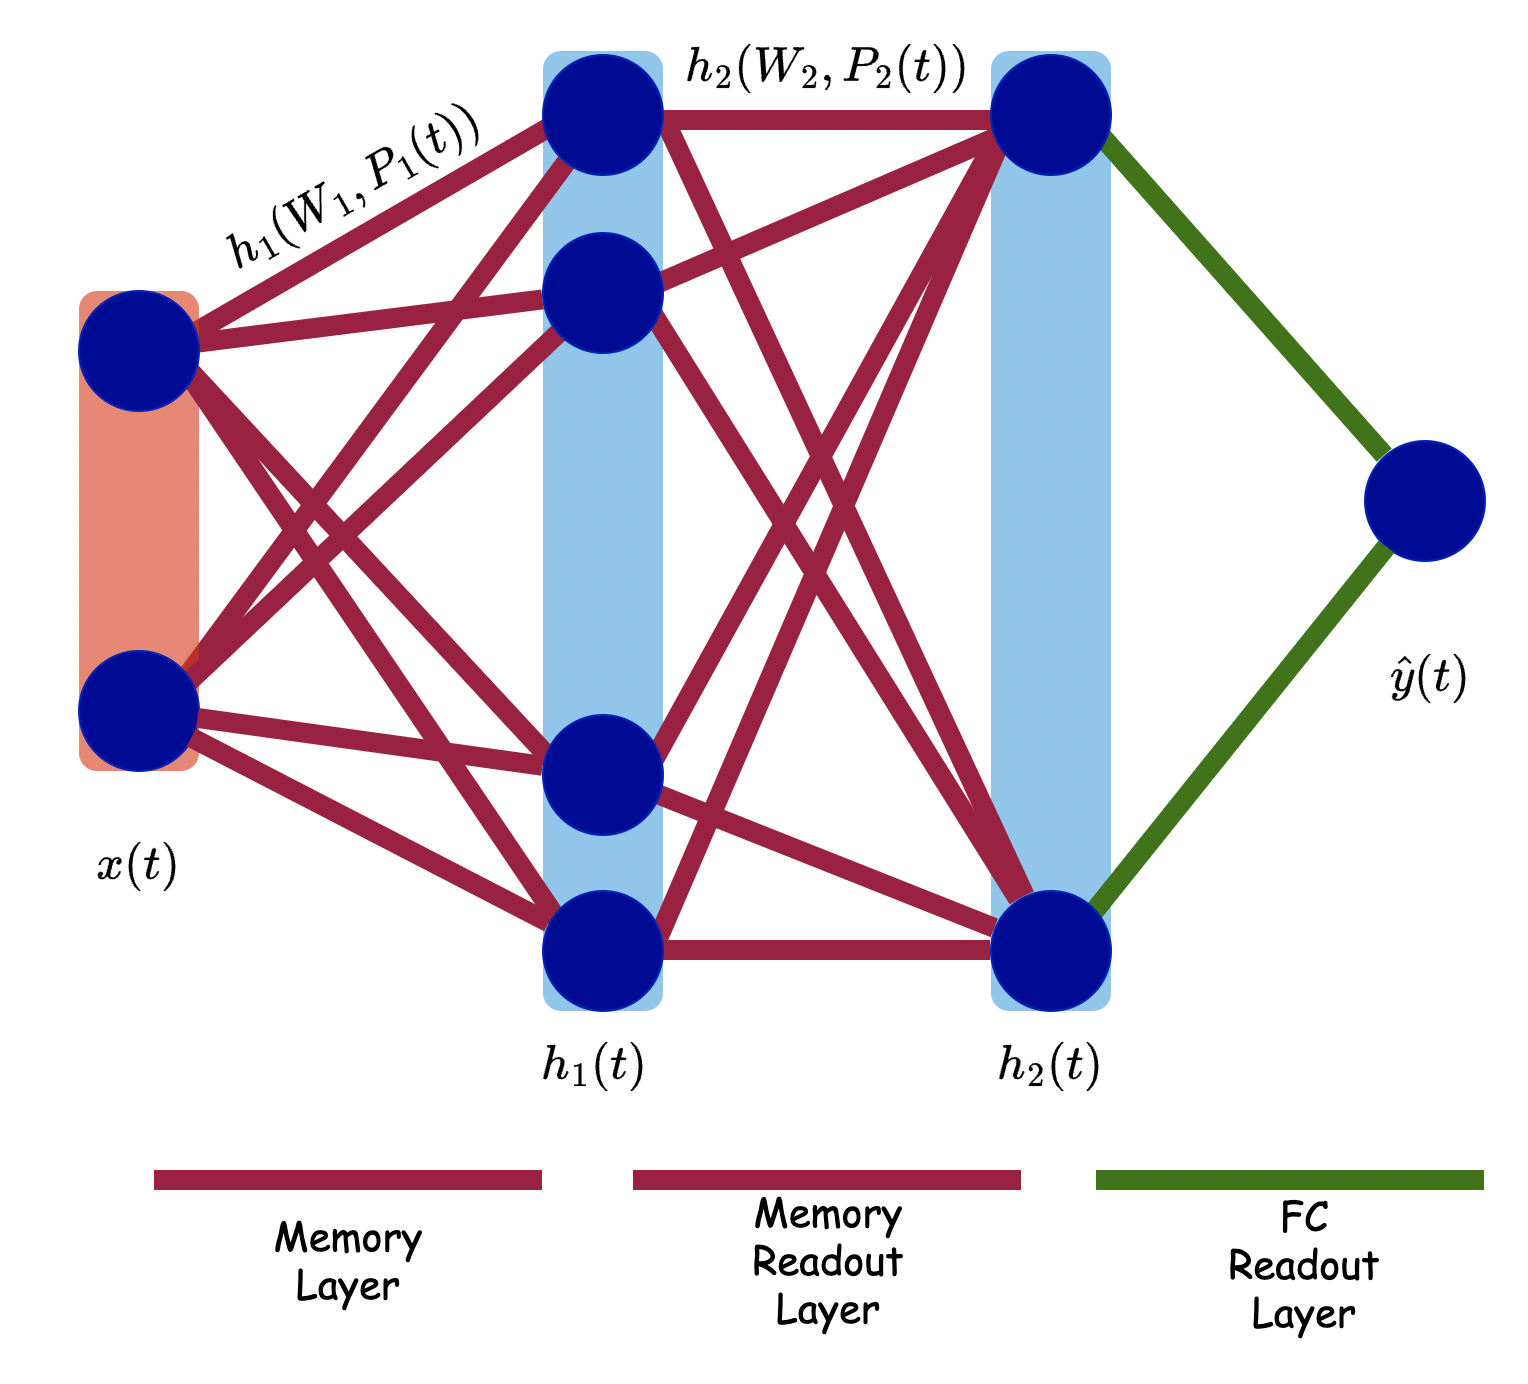
\includegraphics[width=\textwidth]{Memory}
        \caption{Memory Based Readout}
        \label{fig:memory}
    \end{subfigure}
    \hfill
    \begin{subfigure}{0.45\textwidth}
        \centering
        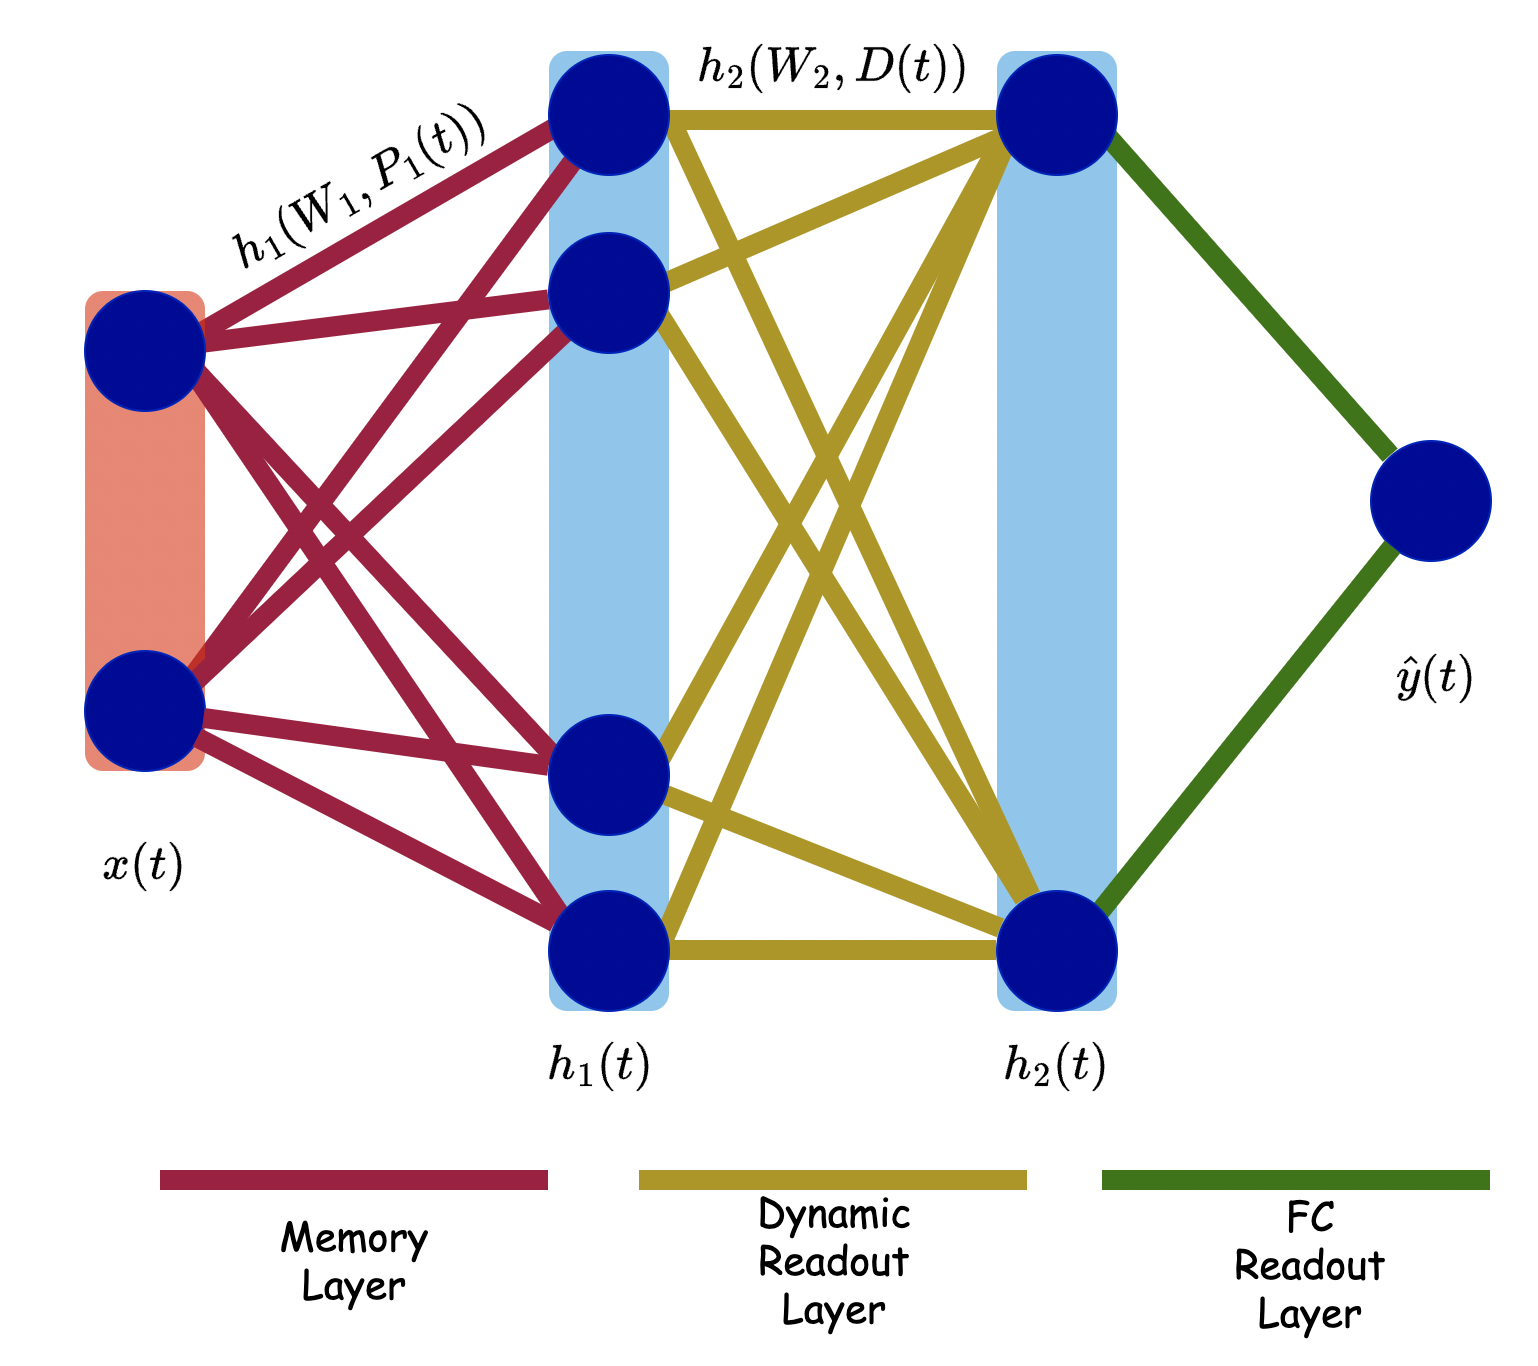
\includegraphics[width=\textwidth]{DynRO}
        \caption{Dynamic Read Out}
        \label{fig:dynro}
    \end{subfigure}
    \caption{The four types of readouts}
    \label{fig:grid}
\end{figure}

For the readout layer, we present four different versions: Fully Connected readout, Nonlinear readout, Memory Based readout, and Dynamic readout:

\begin{itemize}
    \item \textbf{Fully Connected readout (\textbf{FC}):} This version is a plain fully connected layer, represented as follows:
    \begin{equation}
    \sigma\left(\boldsymbol{W_f} \boldsymbol{h_1}(t)+\boldsymbol{b_f}\right)
    \end{equation}
    
    \item \textbf{Nonlinear readout (\textbf{Nonl}):} This version transforms $\boldsymbol{h_1}(t)$ with a nonlinear layer before a FC transformation:
    \begin{align}
    \sigma\left(\boldsymbol{W_2} \boldsymbol{h_1}(t)+\boldsymbol{b_2}\right), \\
    \sigma\left(\boldsymbol{W_f} \boldsymbol{h_2}(t)+\boldsymbol{b_f}\right)
    \end{align}
    
    \item \textbf{Memory Based readout (\textbf{Memo}):} This version leverages the benefit of additional layers of memory for improved performance. This transformation, identical to the one performed by the first memory layer, is denoted by $h_2 = h(\boldsymbol{W_2},\boldsymbol{P_2}(t))$. Subsequently, we apply the same FC layer transformation:

\begin{equation}
\sigma\left(\boldsymbol{W_f} \boldsymbol{h_2}(t)+\boldsymbol{b_f}\right)
\end{equation}

\item \textbf{Dynamic readout (\textbf{Dyn}):} This version is inspired by the observation that the decay rate $\lambda$ in \textbf{Memo} is extremely low, which signifies minimal memory retention. \textbf{Dyn} addresses this issue by modifying the update rule for the plasticity matrix as follows:
\begin{equation}
\boldsymbol{P}(t)= \boldsymbol{\eta} \odot\left(\boldsymbol{h_1}(t) \boldsymbol{x}(t)^T\right)
\end{equation}

This change results in a dynamic readout of the current time step. Apart from this modification, everything else in \textbf{Dyn} mirrors \textbf{Memo}. The dynamic transition is denoted by $h_2 = h(\boldsymbol{W_2},\boldsymbol{D}(t))$. Following this, the same FC layer transformation is applied:
\begin{equation}
\sigma\left(\boldsymbol{W_f} \boldsymbol{h_2}(t)+\boldsymbol{b_f}\right)
\end{equation}
\end{itemize}



\section{Results \& Analysis}

\subsection{overall comparision}

To maintain an equitable comparison, we constrain the number of dynamic neurons to be equivalent across all models. In our investigation, we considered models with dynamic neuron counts of $50$ and $100$. Their respective performance metrics are detailed in the table below:

\begin{table}[!ht]
    \centering
    \renewcommand{\arraystretch}{1.5}  % Vertical padding
    \begin{tabular}{|c|c|c|c|c|c|c|c|c|c|c|c|c|c|}
    \hline
        \multicolumn{14}{|c|}{\textbf{Max R}} \\ \hline
        & \multicolumn{6}{c|}{\textbf{M}} & \multicolumn{6}{c|}{\textbf{A}} & \textbf{\textbf{Stack}} \\ \cline{2-14}
        \diagbox[width=10em]{\raisebox{2ex}{Size}}{\raisebox{-1ex}{Net}} & \multirow{2}{*}{\centering \textbf{FC}} & \multirow{2}{*}{\centering \textbf{Nonl}} & \multicolumn{2}{c|}{\textbf{Dyn}} & \multicolumn{2}{c|}{\textbf{Memo}} & \multirow{2}{*}{\centering \textbf{FC}} & \multirow{2}{*}{\centering \textbf{Nonl}} & \multicolumn{2}{c|}{\textbf{Dyn}} & \multicolumn{2}{c|}{\textbf{Memo}} & \multirow{2}{*}{\centering \textbf{FC}} \\ \cline{4-7}\cline{10-13}
        & & & \textbf{M} & \textbf{A} & \textbf{M} & \textbf{A} & & & \textbf{M} & \textbf{A} & \textbf{M} & \textbf{A} & \\ \hline
        50 & 5 & 7 & 9 & 9 & 8& 9 & 6 & 4 & 4 & 4 & 4 & 4 & 6 \\ \hline
        100 & 9 & 10 & 12 & 13 & 9 & 14 & 9 & 7 & 5 & 5 & 5 & 5 & 7 \\ \hline
    \end{tabular}
\caption{Performance metrics for different dynamic neuron sizes}
\label{tbl:performance_metrics}
\end{table}

Analyzing the table, we can deduce the following:

\begin{enumerate}
\item Across most types of readouts, \textbf{M} outperforms \textbf{A}.
\item \textbf{M} benefits from more intricate readouts and scaling. Conversely, the performance of \textbf{A} diminishes with more complex readouts.
\item The most noteworthy performance is achieved by the memory layer of \textbf{M}, combined with either \textbf{Dyn} or \textbf{Memo} readout layers.
\end{enumerate}

A graph of performance is here:
\begin{figure}[h!]
\includegraphics[width=1\textwidth]{all_p}
\caption{Performance across all networks and sizes}
\end{figure}

\section{M vs A}
In this section, we address the possible reasons why multiplicative plasticity matrix has a better performance.
From the graph below, we can see that a complex readout hurts the performance of A networks, whereas a complex readout helps the performance of M networks. 
\begin{figure}[h!]
\includegraphics[width=1\textwidth]{MvA.png}
\caption{M vs A}
\end{figure}

To figure out why the network works, we plot the hidden layer activities across time, the eta matrix, the weight matrix, the actual weight/plasticity across time. Specifically, we choose the \textbf{Memo} Network with \textbf{M} memory and \textbf{A} readout:

\begin{figure}[h!]
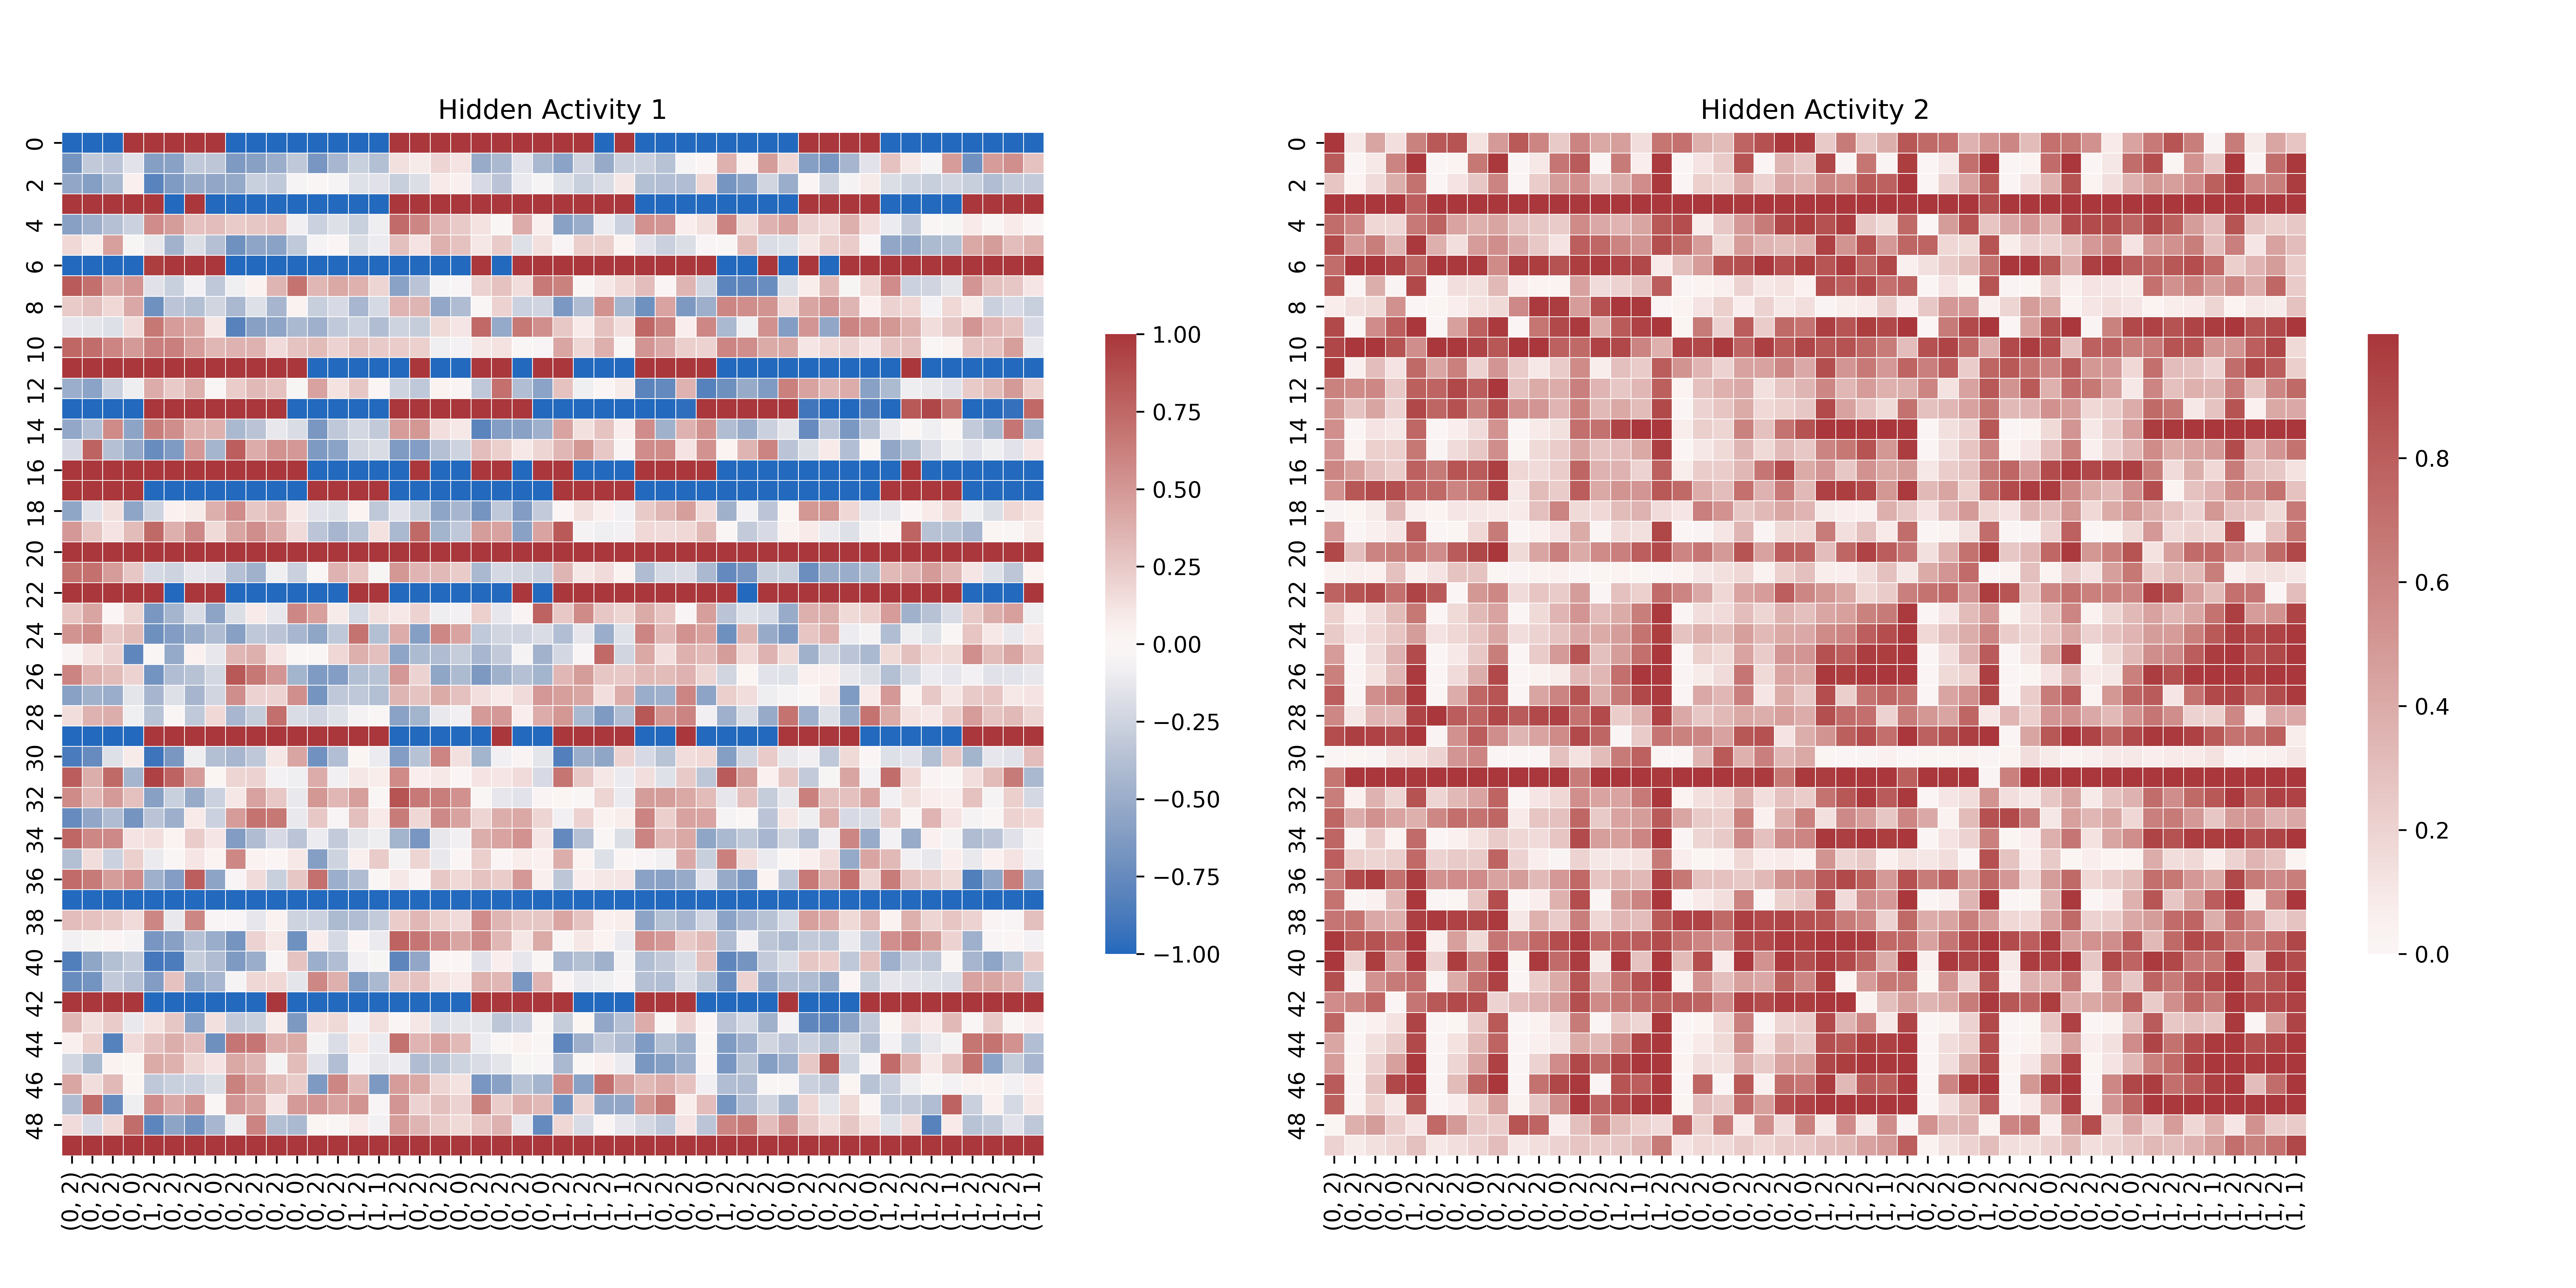
\includegraphics[width=1\textwidth]{HL_Combined}
\caption{Hidden Layers Across Time}
\end{figure}

\begin{figure}[h!]
  \centering
  \begin{subfigure}[b]{0.45\textwidth}
    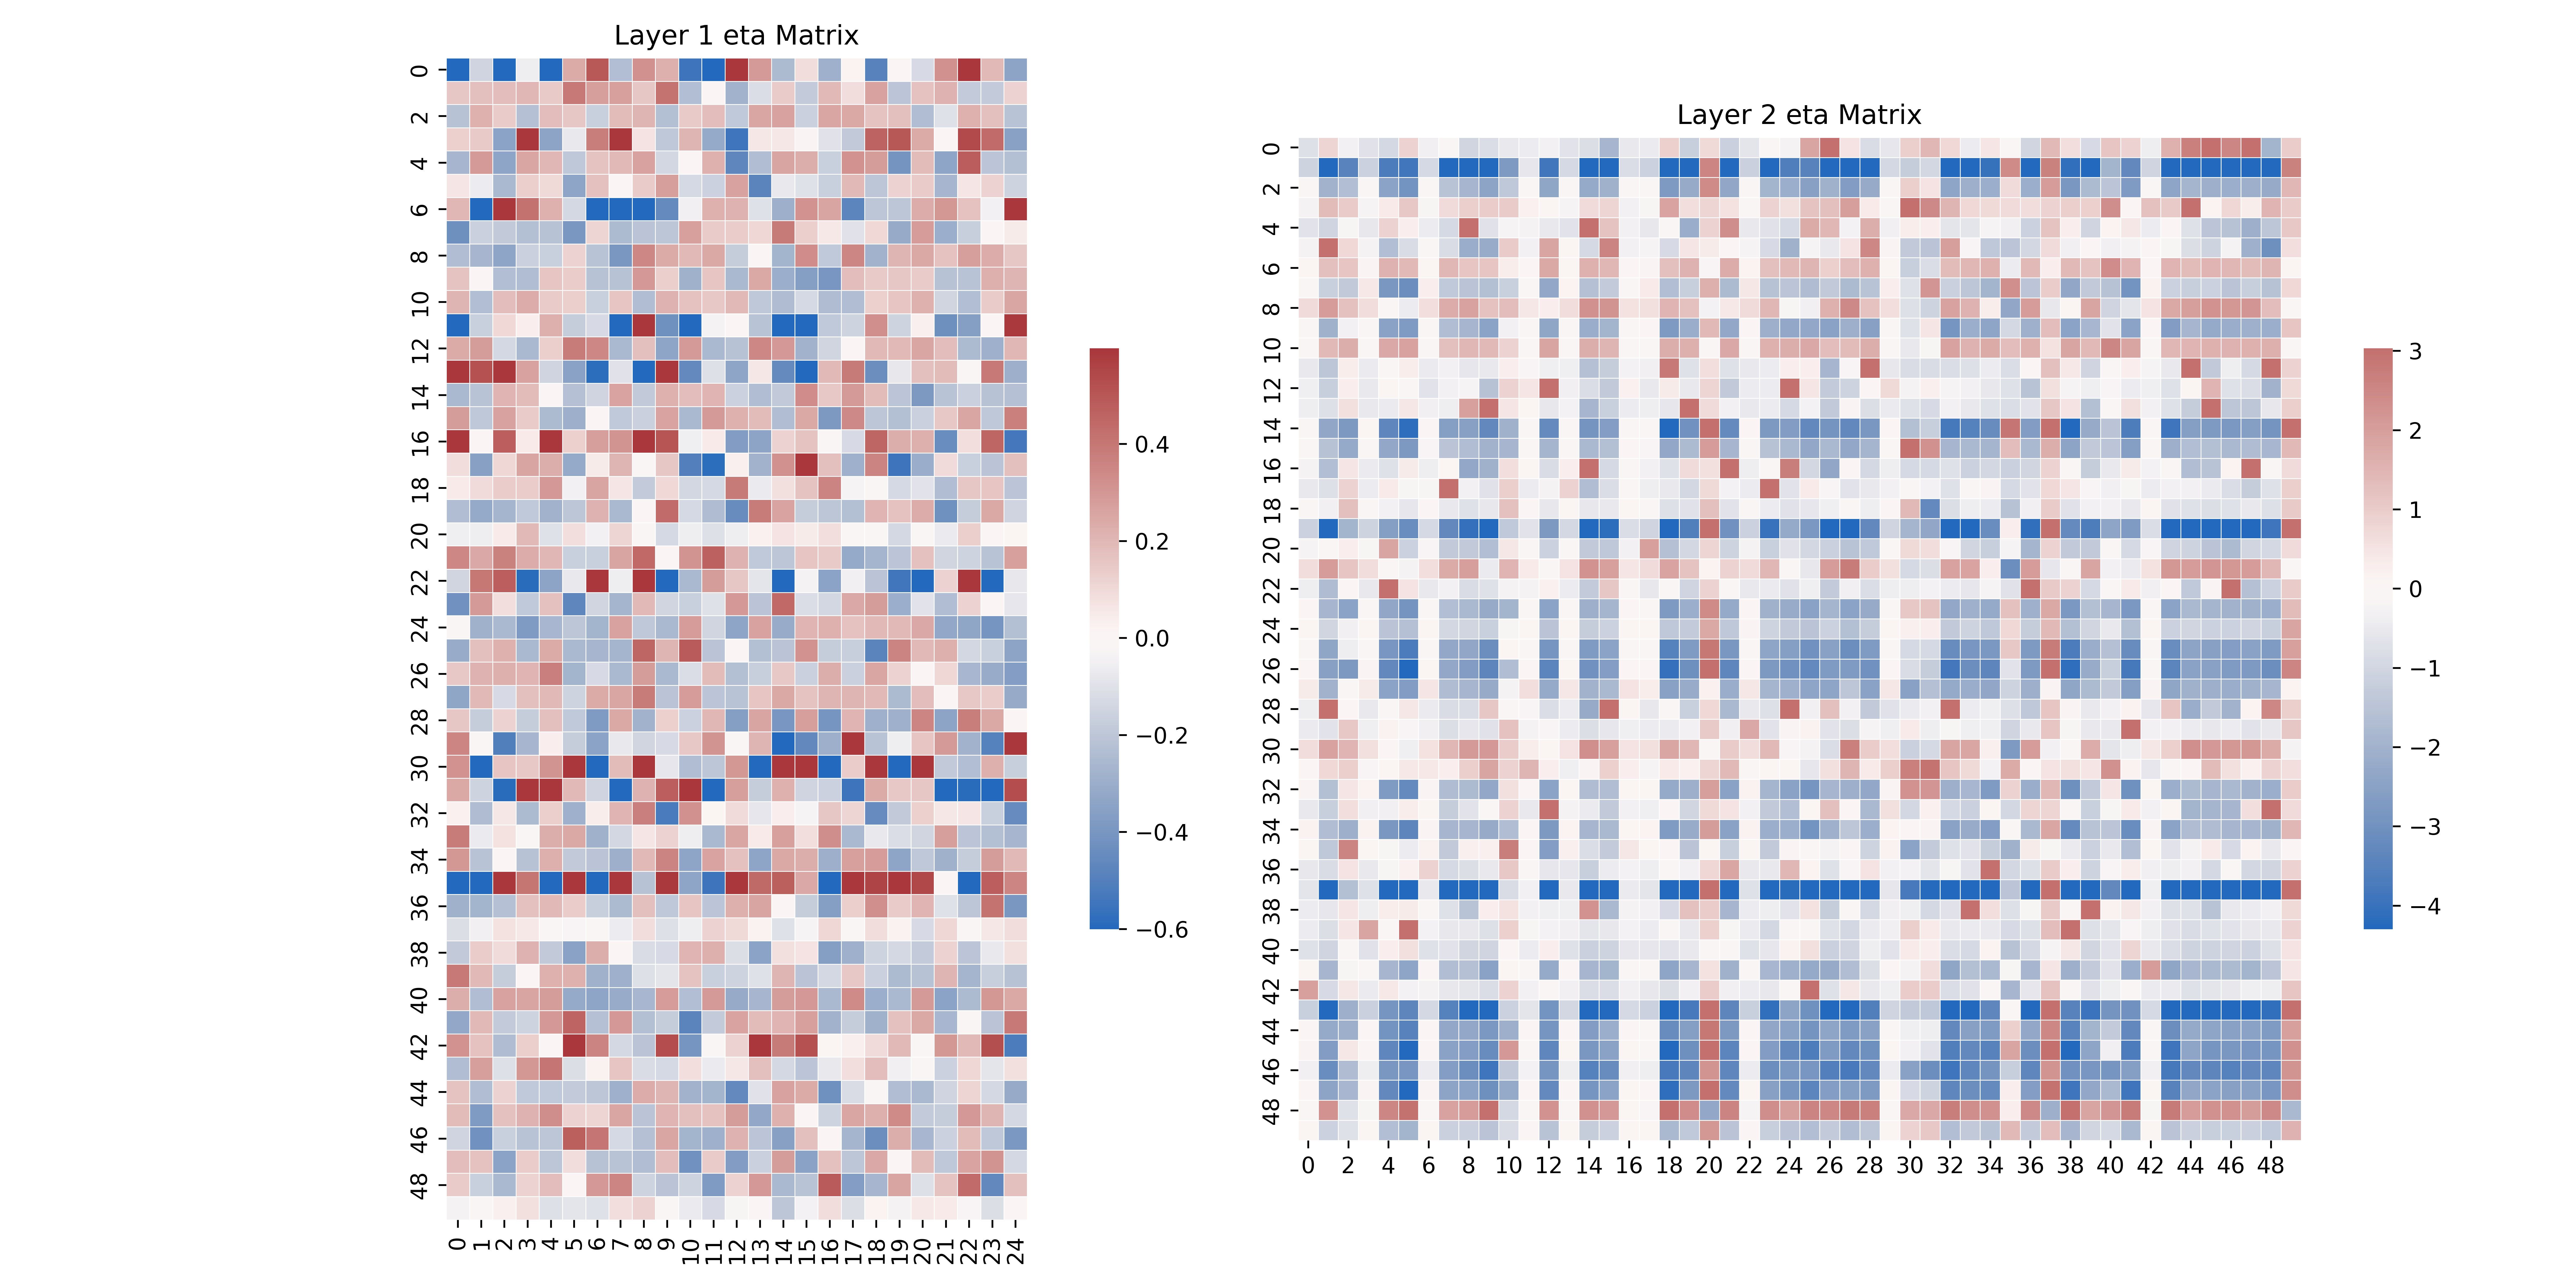
\includegraphics[width=\textwidth]{Eta_Matrices}
    \caption{eta matrix of \textbf{Memo} \textbf{M} \textbf{A} 50/50}
  \end{subfigure}
  \hfill
  \begin{subfigure}[b]{0.45\textwidth}
    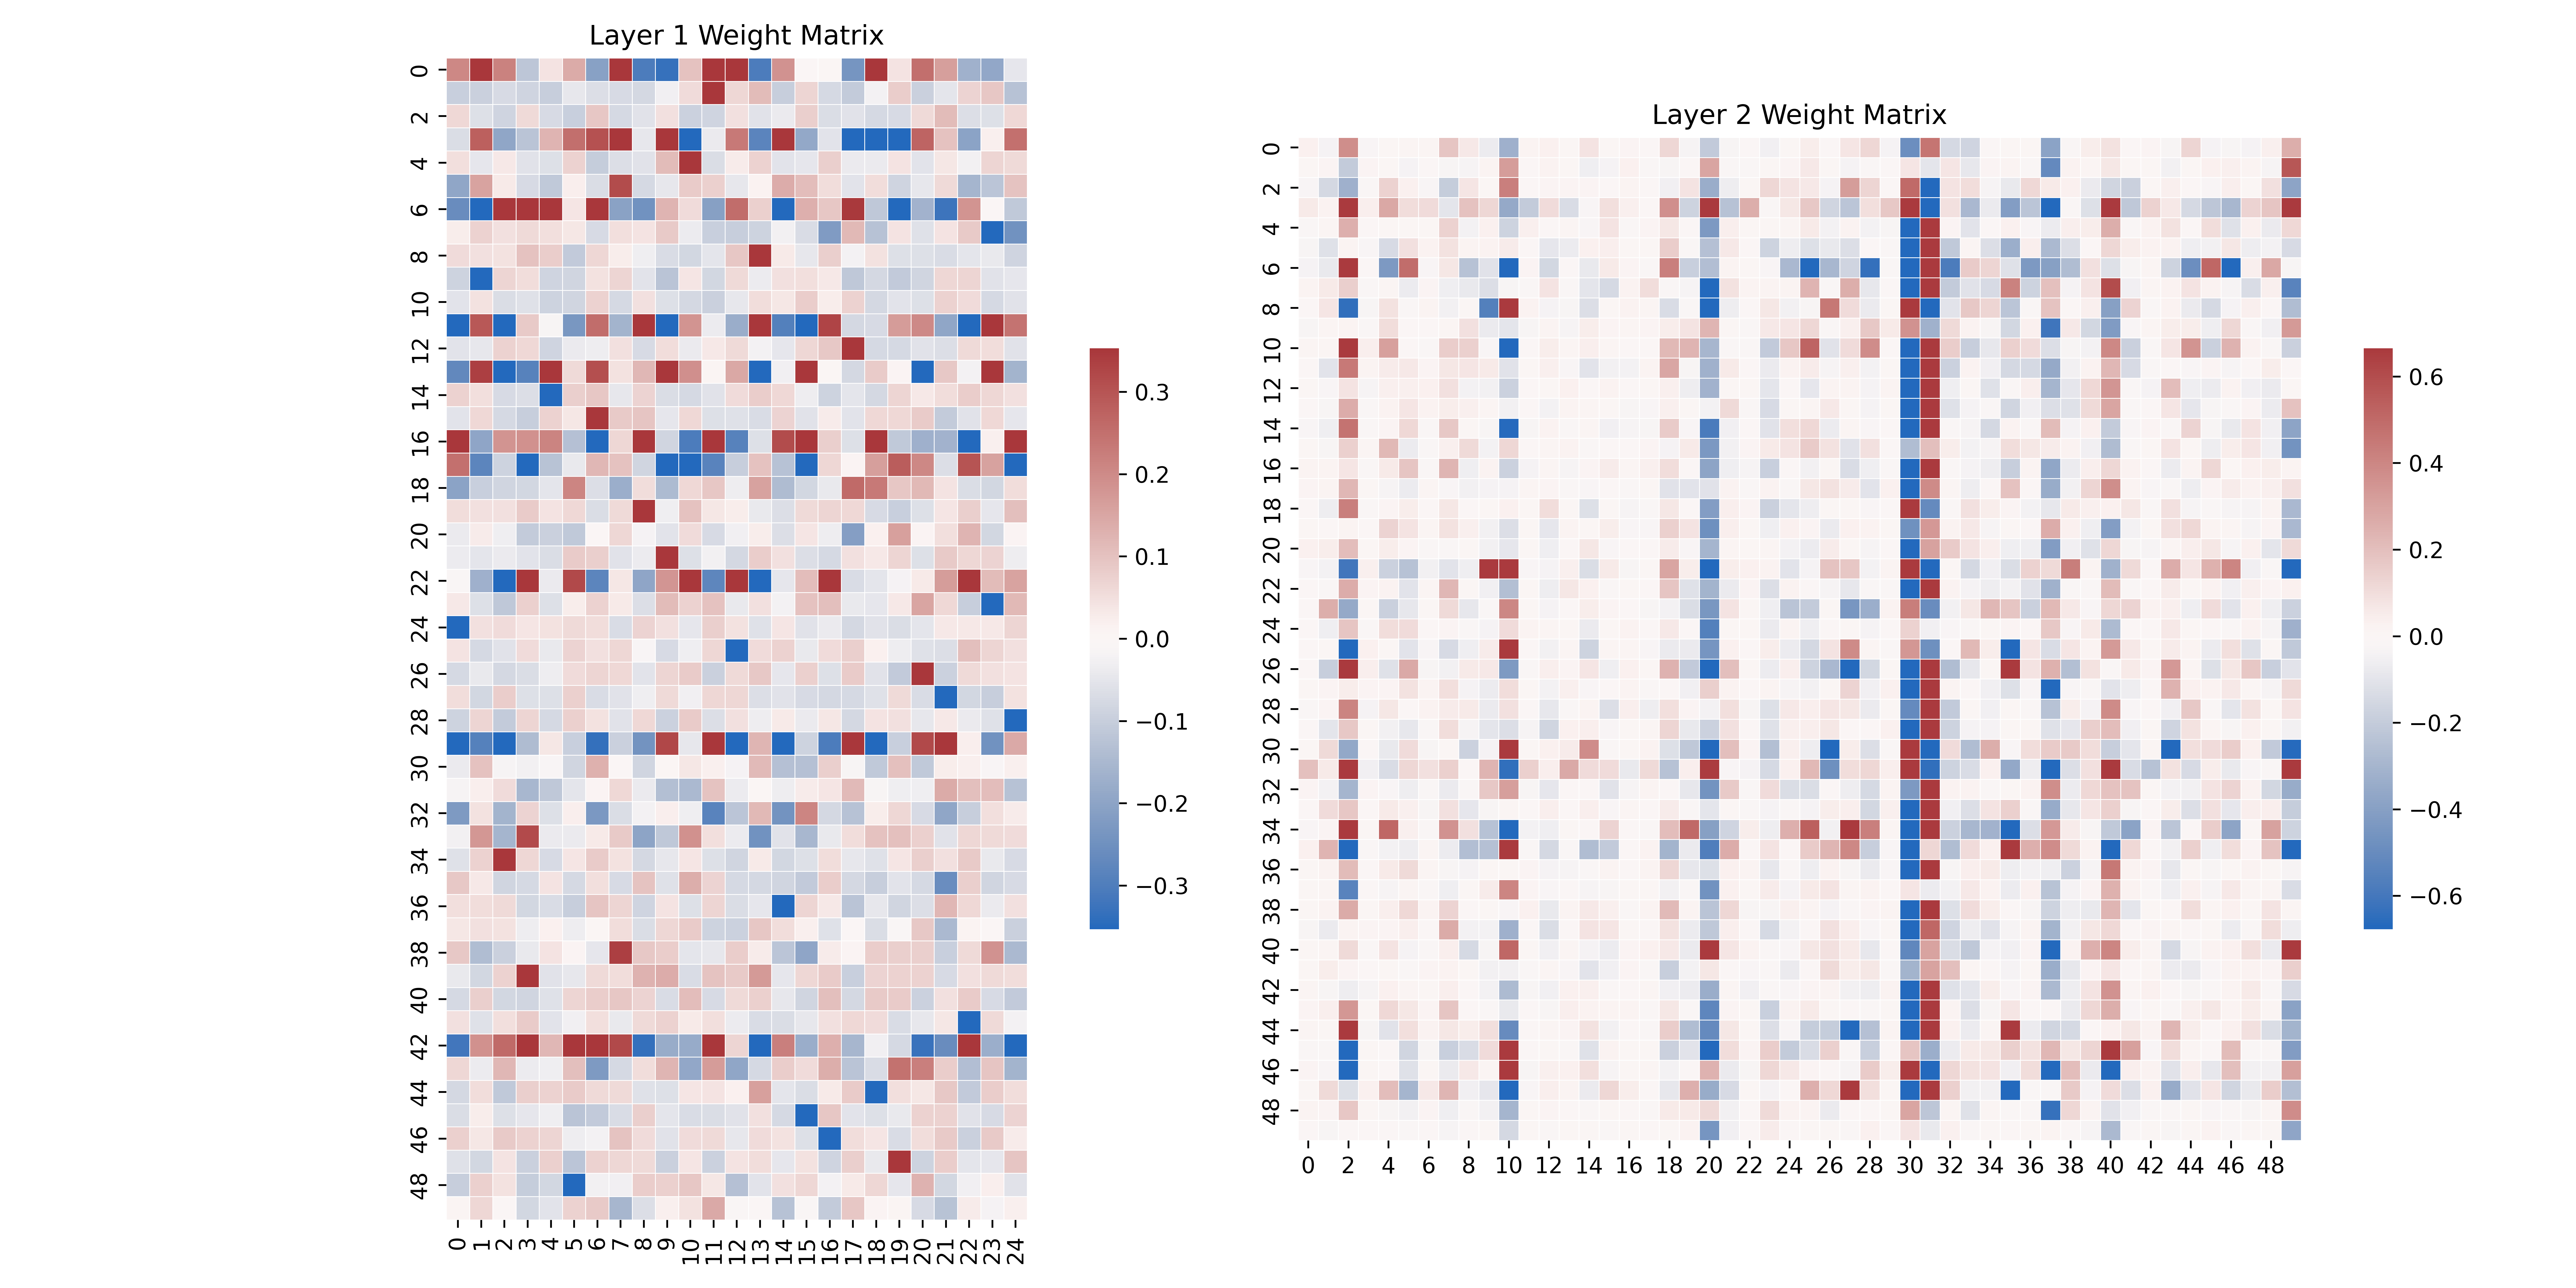
\includegraphics[width=\textwidth]{Weight_Matrices}
    \caption{weight matrix of \textbf{Memo} \textbf{M} \textbf{A} 50/50}
  \end{subfigure}
  \caption{Dyn RO MA 50/50}
\end{figure}

We plot the actual weight and the plasticity matrix with $t$ from 74-77, where at 74,75 the network output 0 and 76,77 the network output 1:
\begin{figure}[h!]
  \centering
  \begin{minipage}[b]{0.45\linewidth}
    \centering
    \begin{subfigure}[b]{\linewidth}
      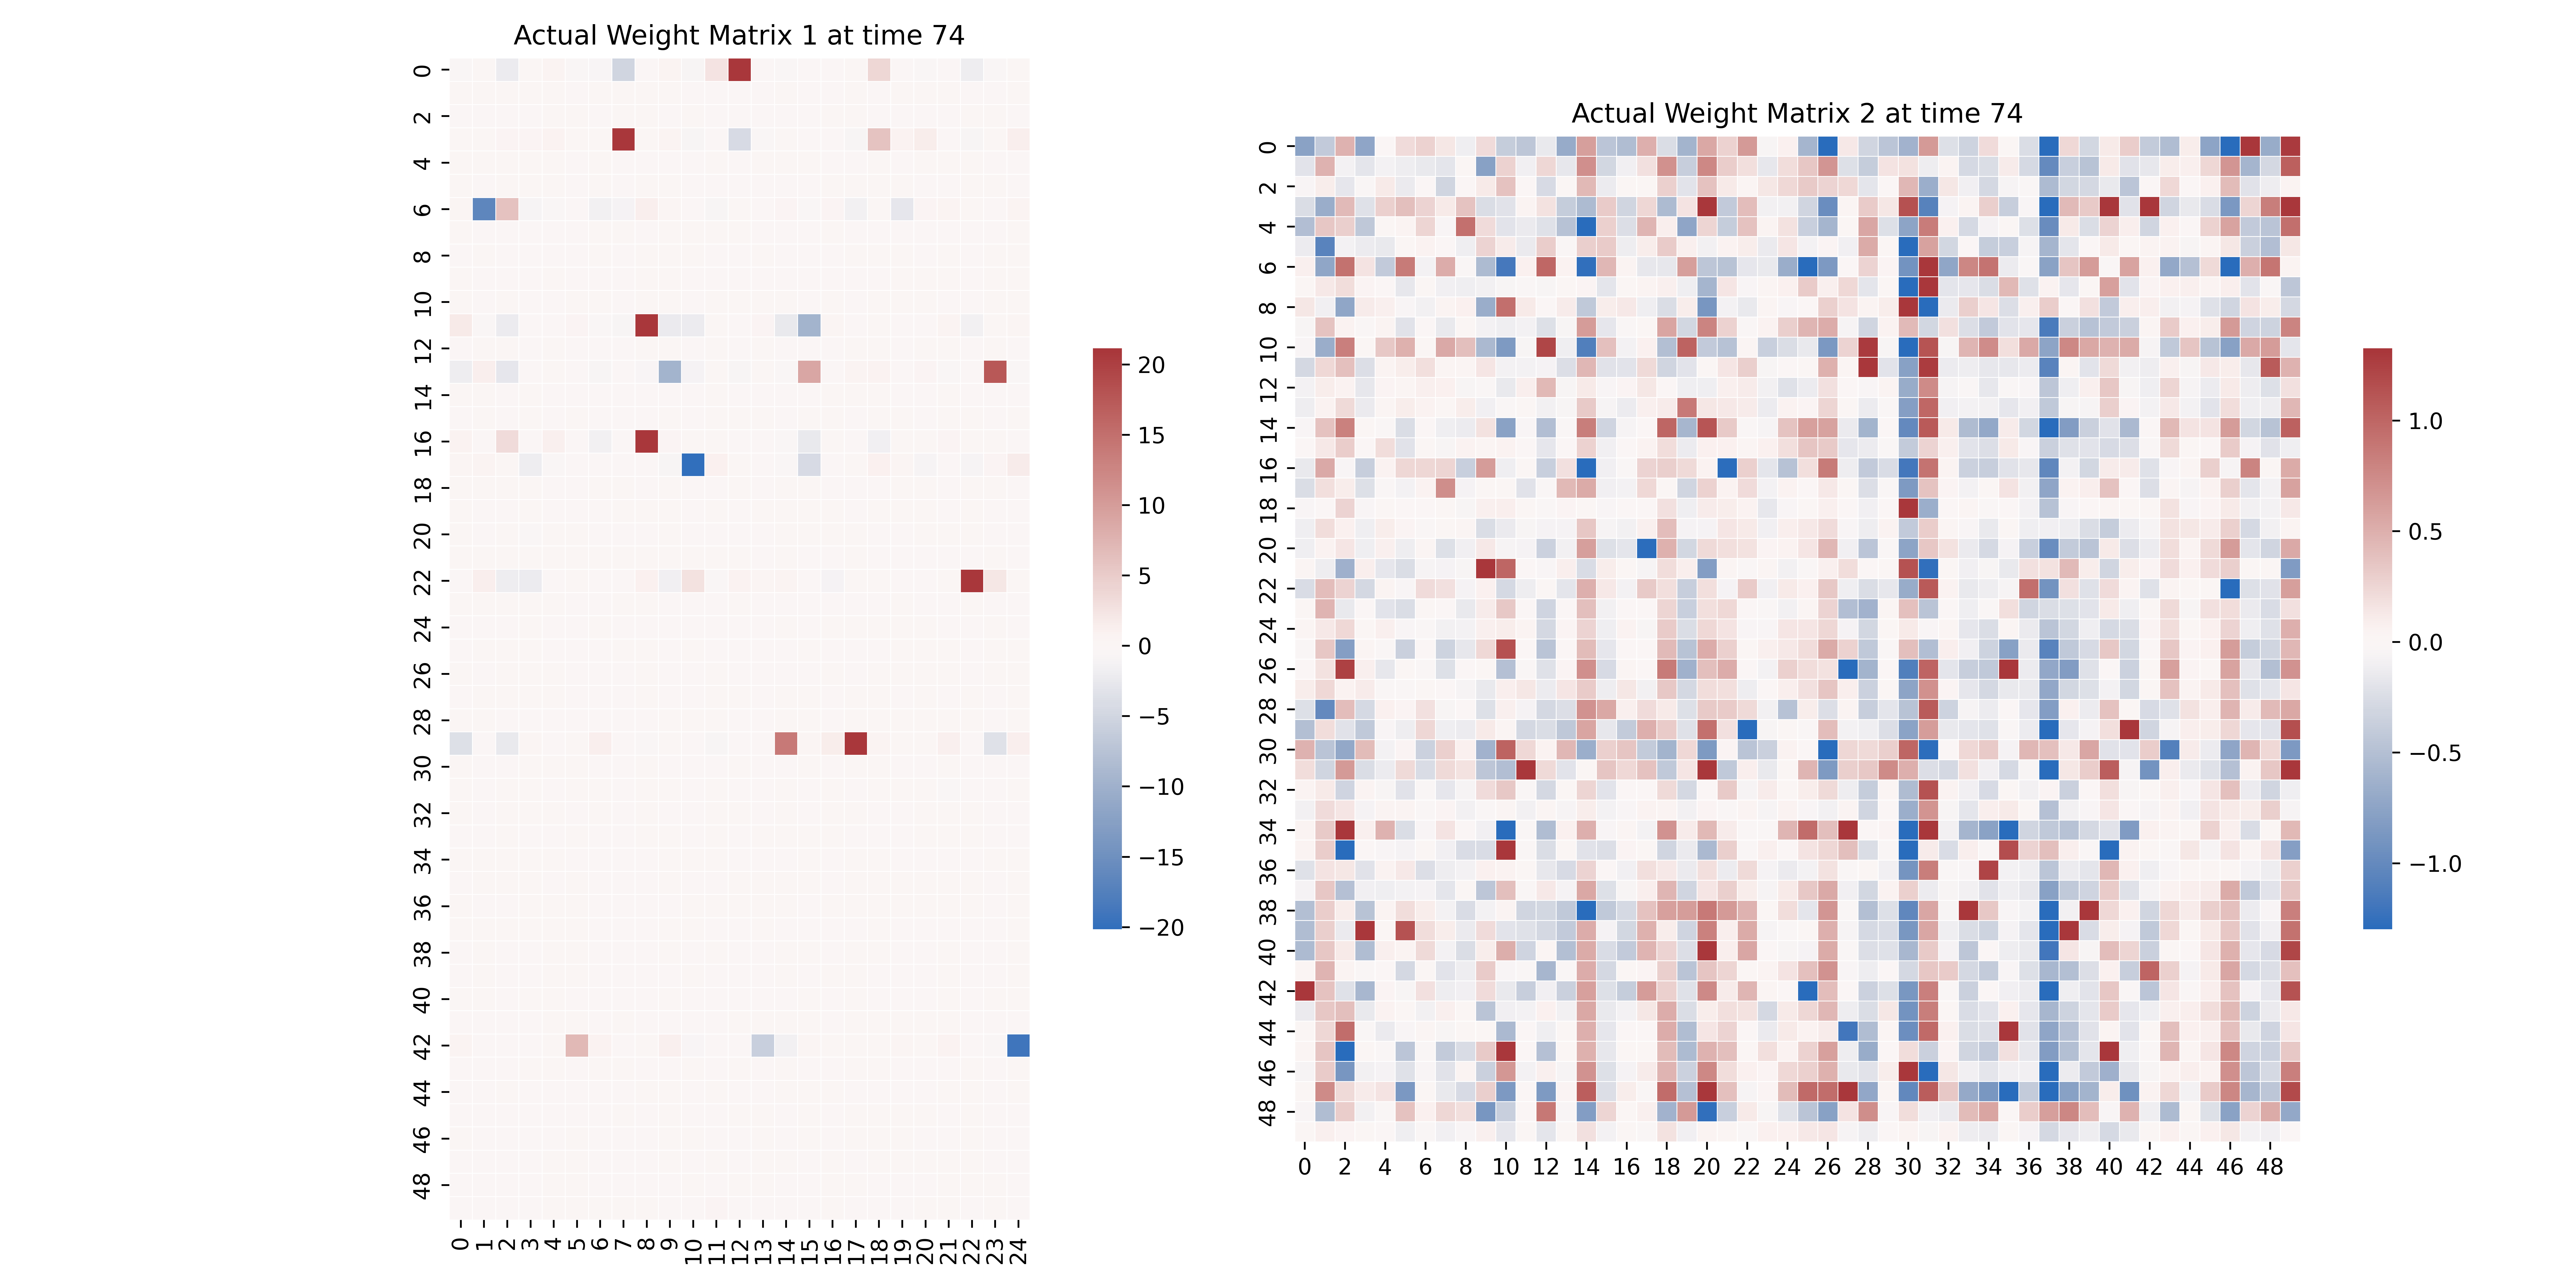
\includegraphics[width=\textwidth]{Actual_Weight_combined_74}
      \caption{T=74}
    \end{subfigure}
    \vfill
    \begin{subfigure}[b]{\linewidth}
      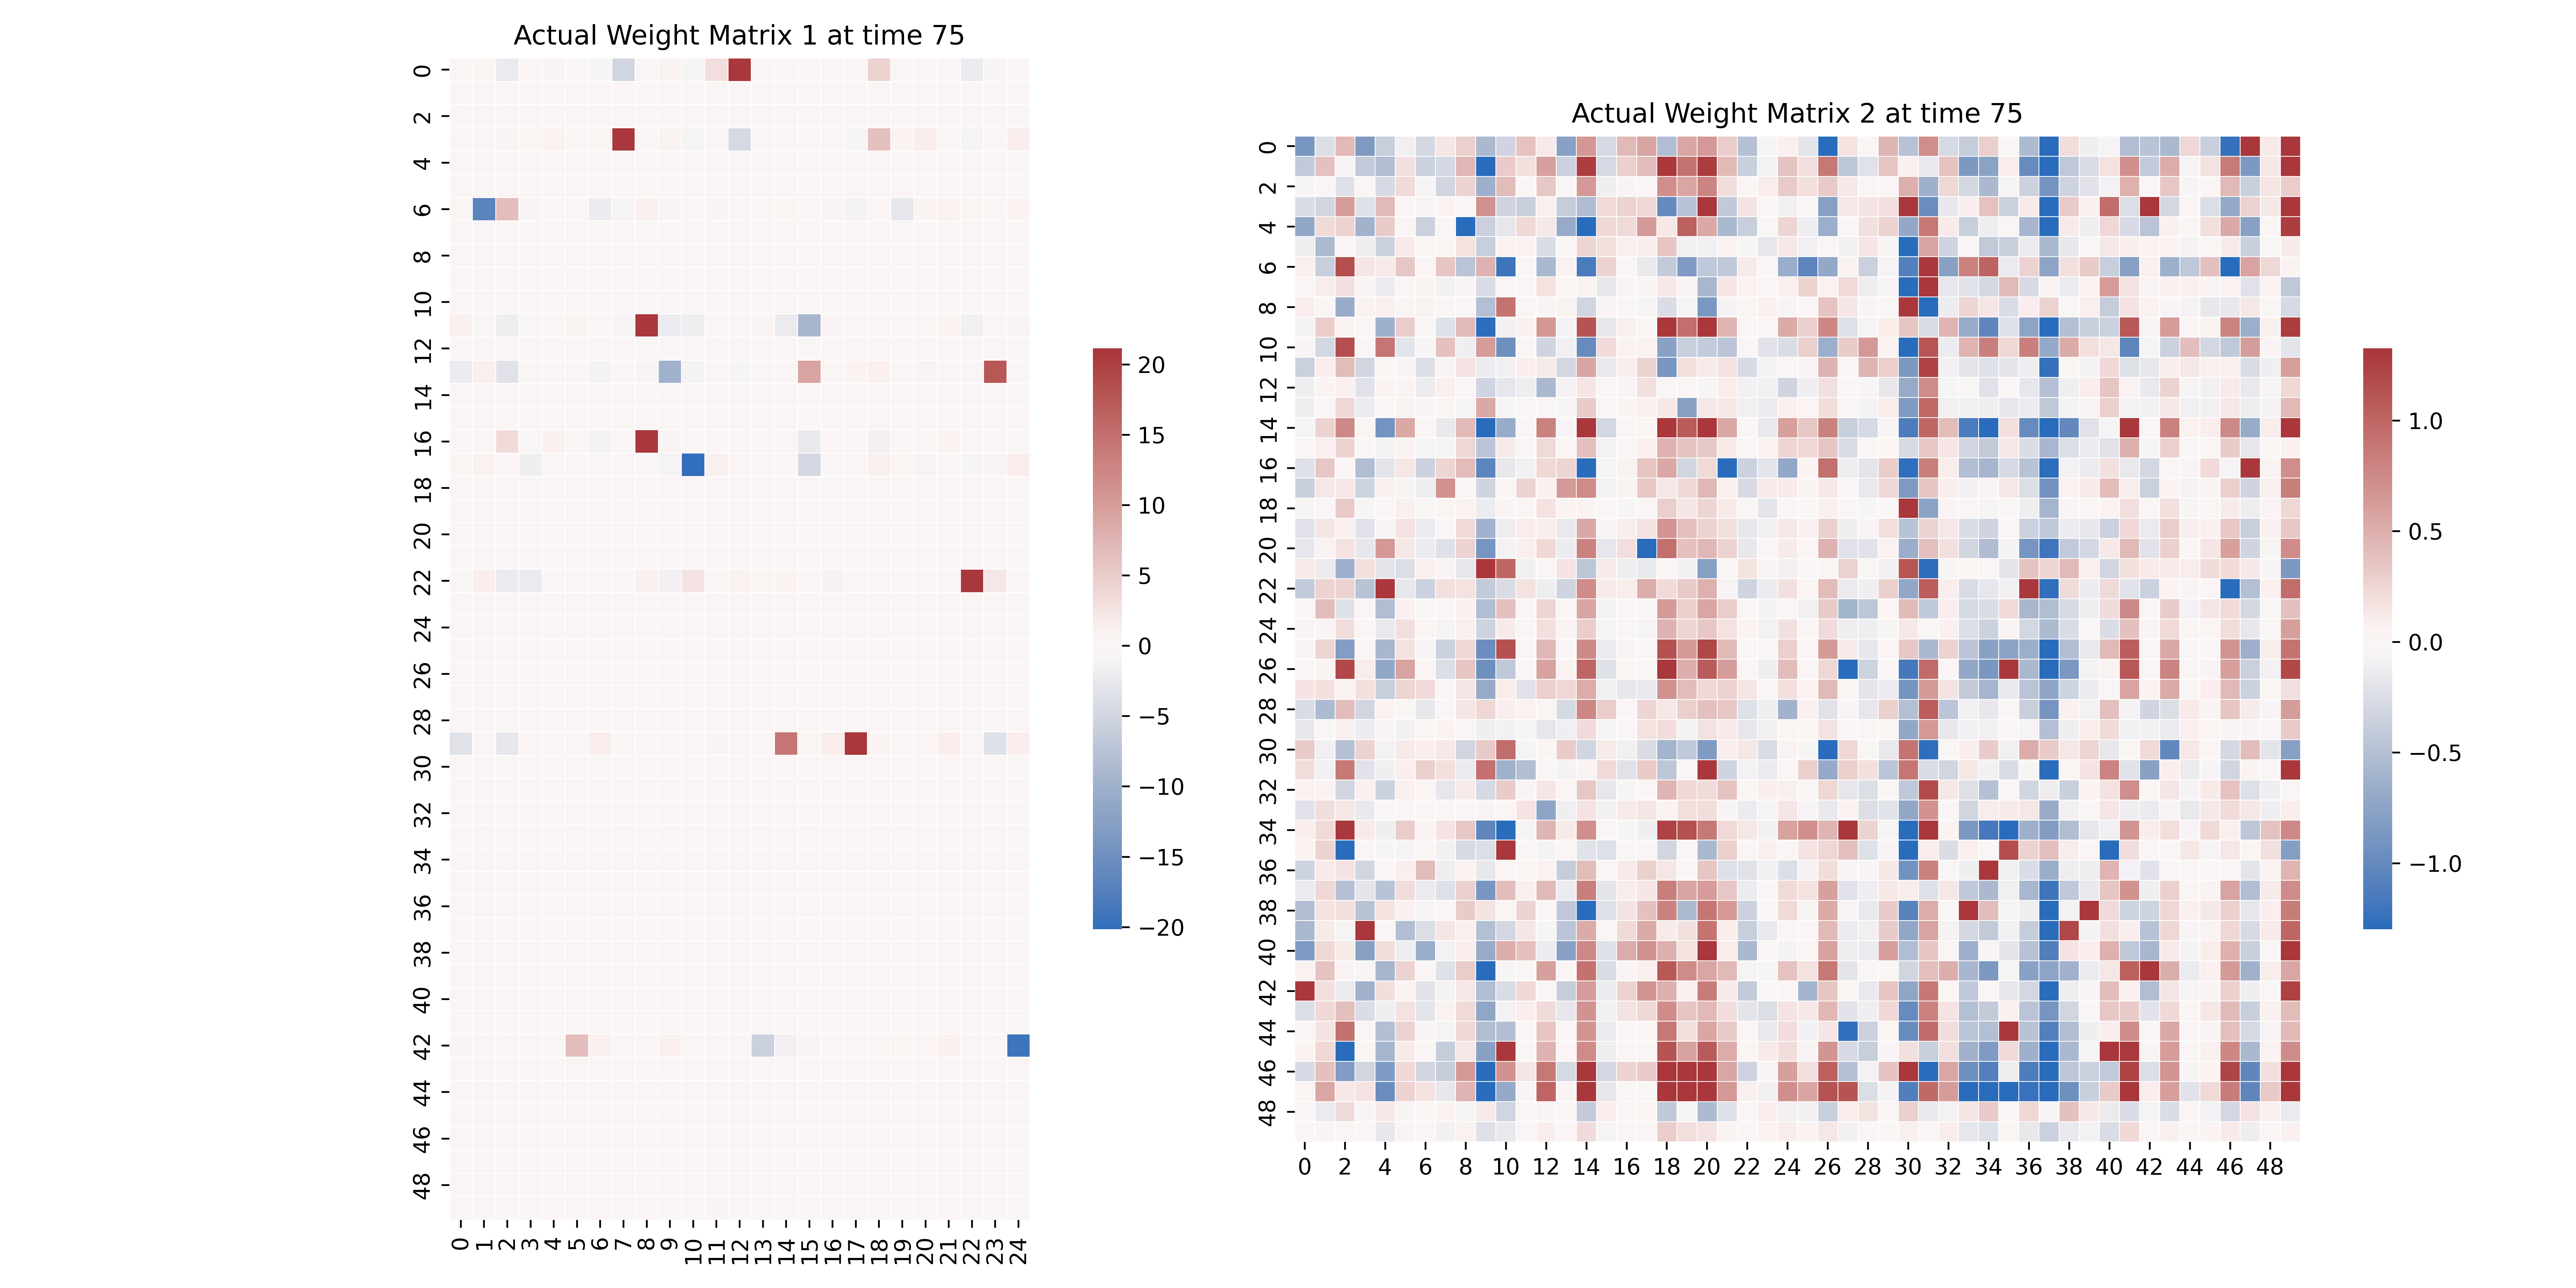
\includegraphics[width=\textwidth]{Actual_Weight_combined_75}
      \caption{T=75}
    \end{subfigure}
  \end{minipage}
  \hfill
  \begin{minipage}[b]{0.45\linewidth}
    \centering
    \begin{subfigure}[b]{\linewidth}
      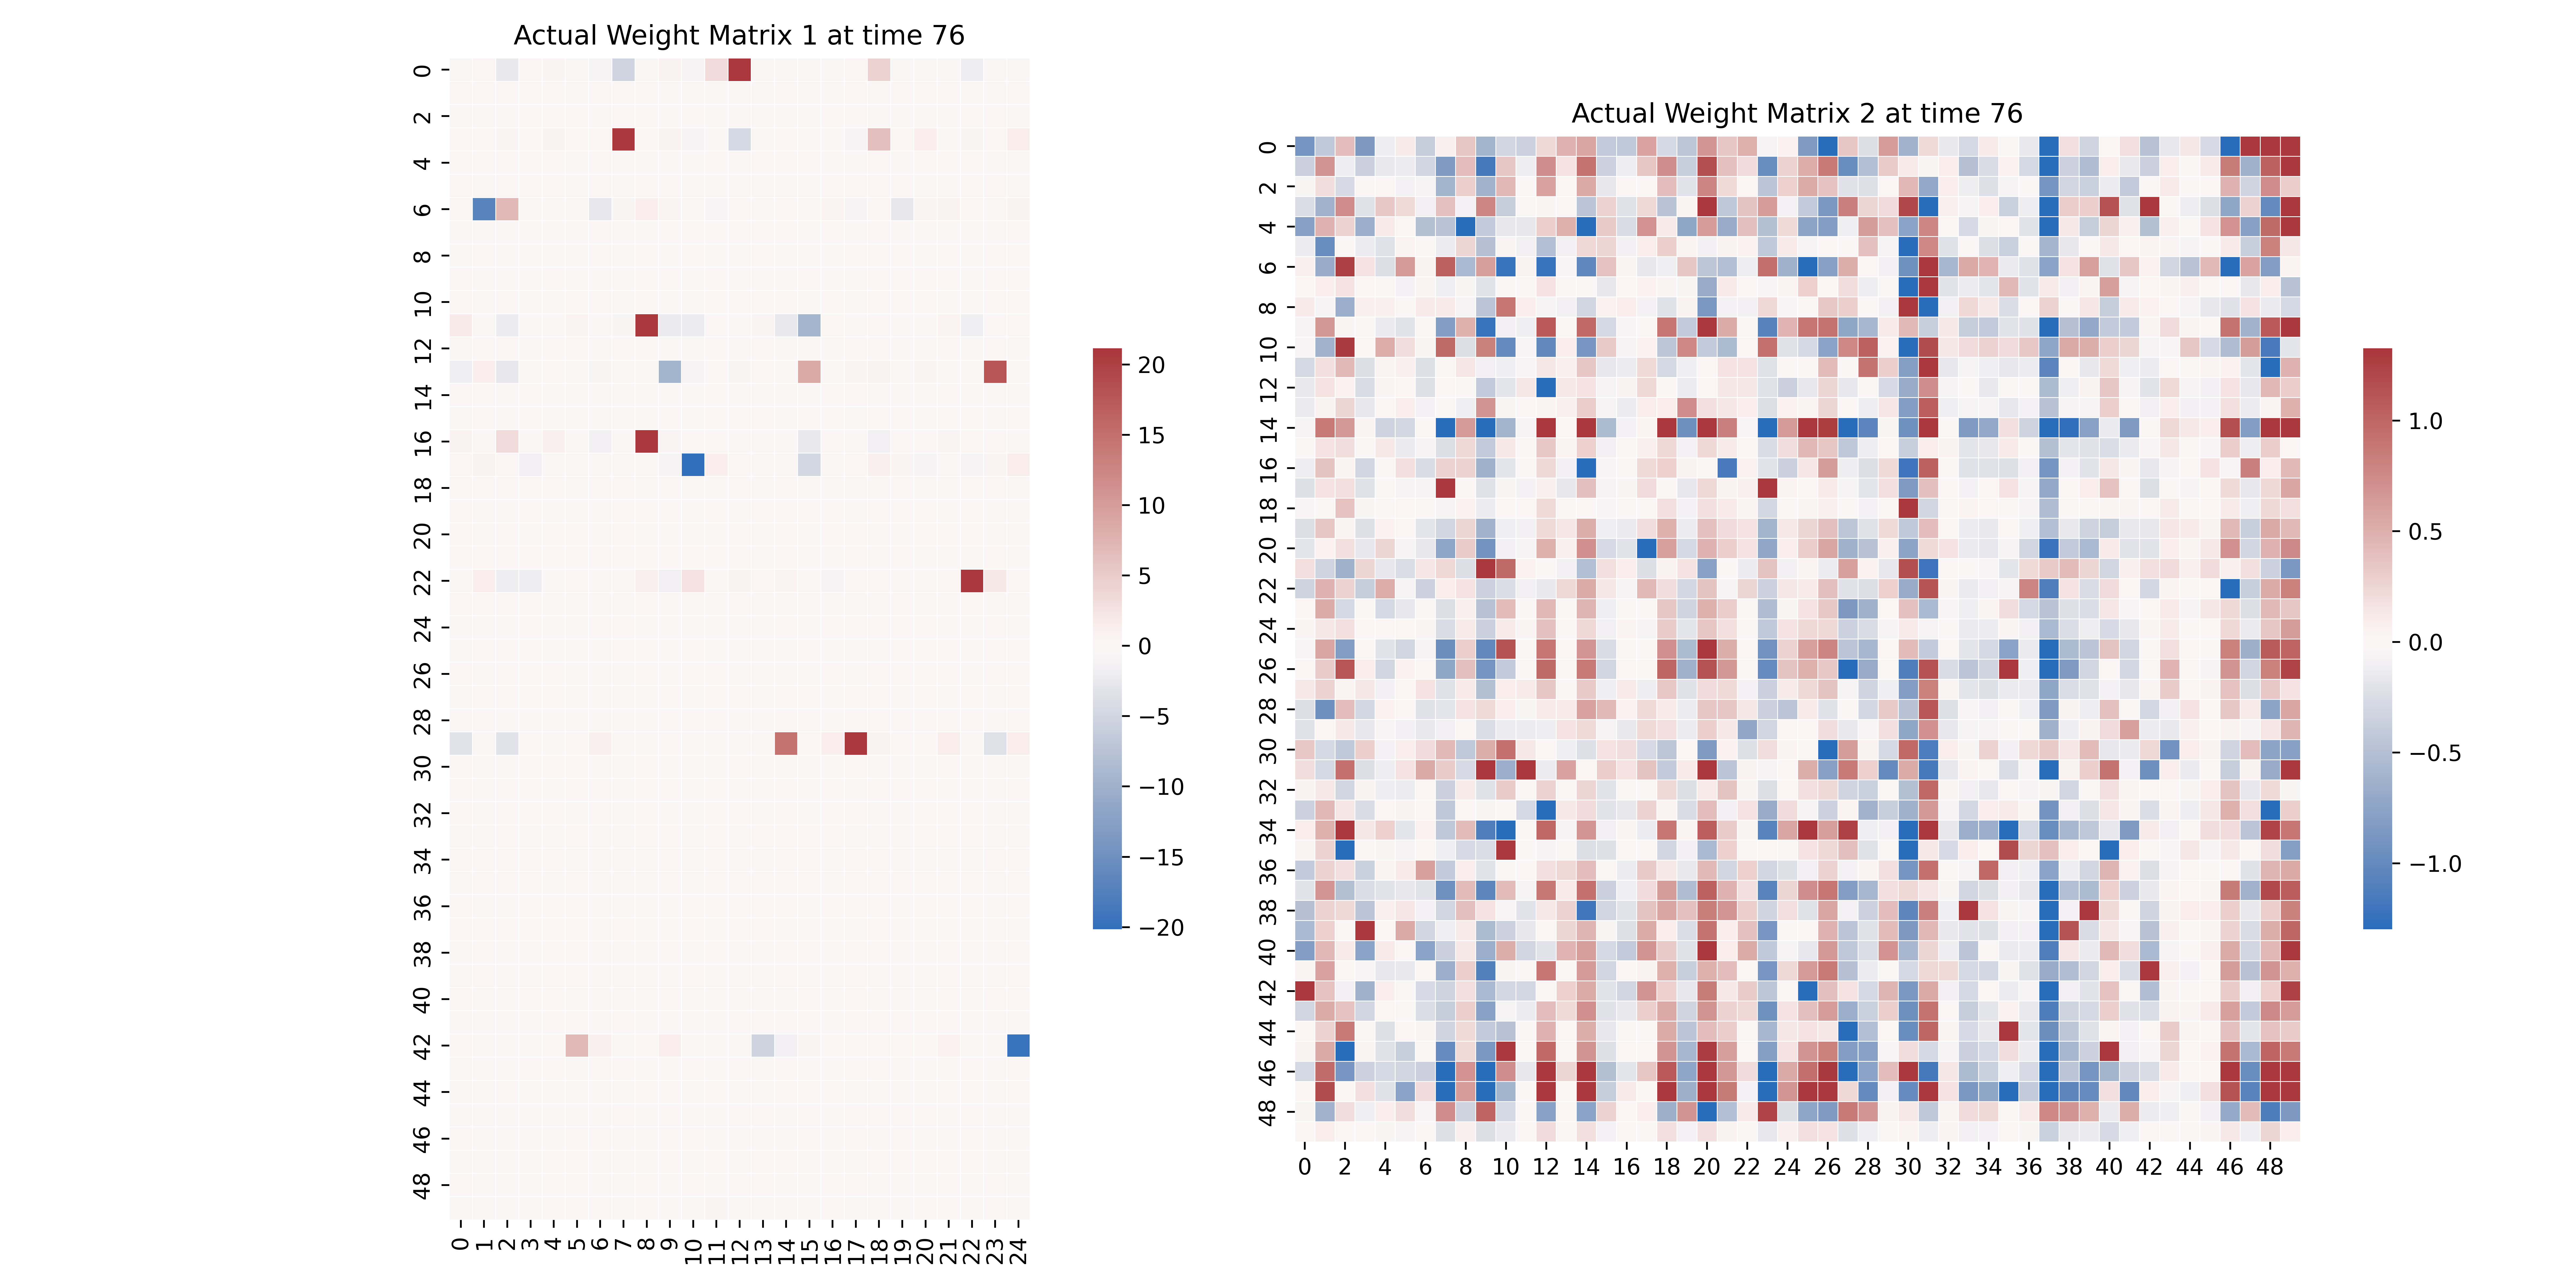
\includegraphics[width=\textwidth]{Actual_Weight_combined_76}
      \caption{T=76}
    \end{subfigure}
    \vfill
    \begin{subfigure}[b]{\linewidth}
      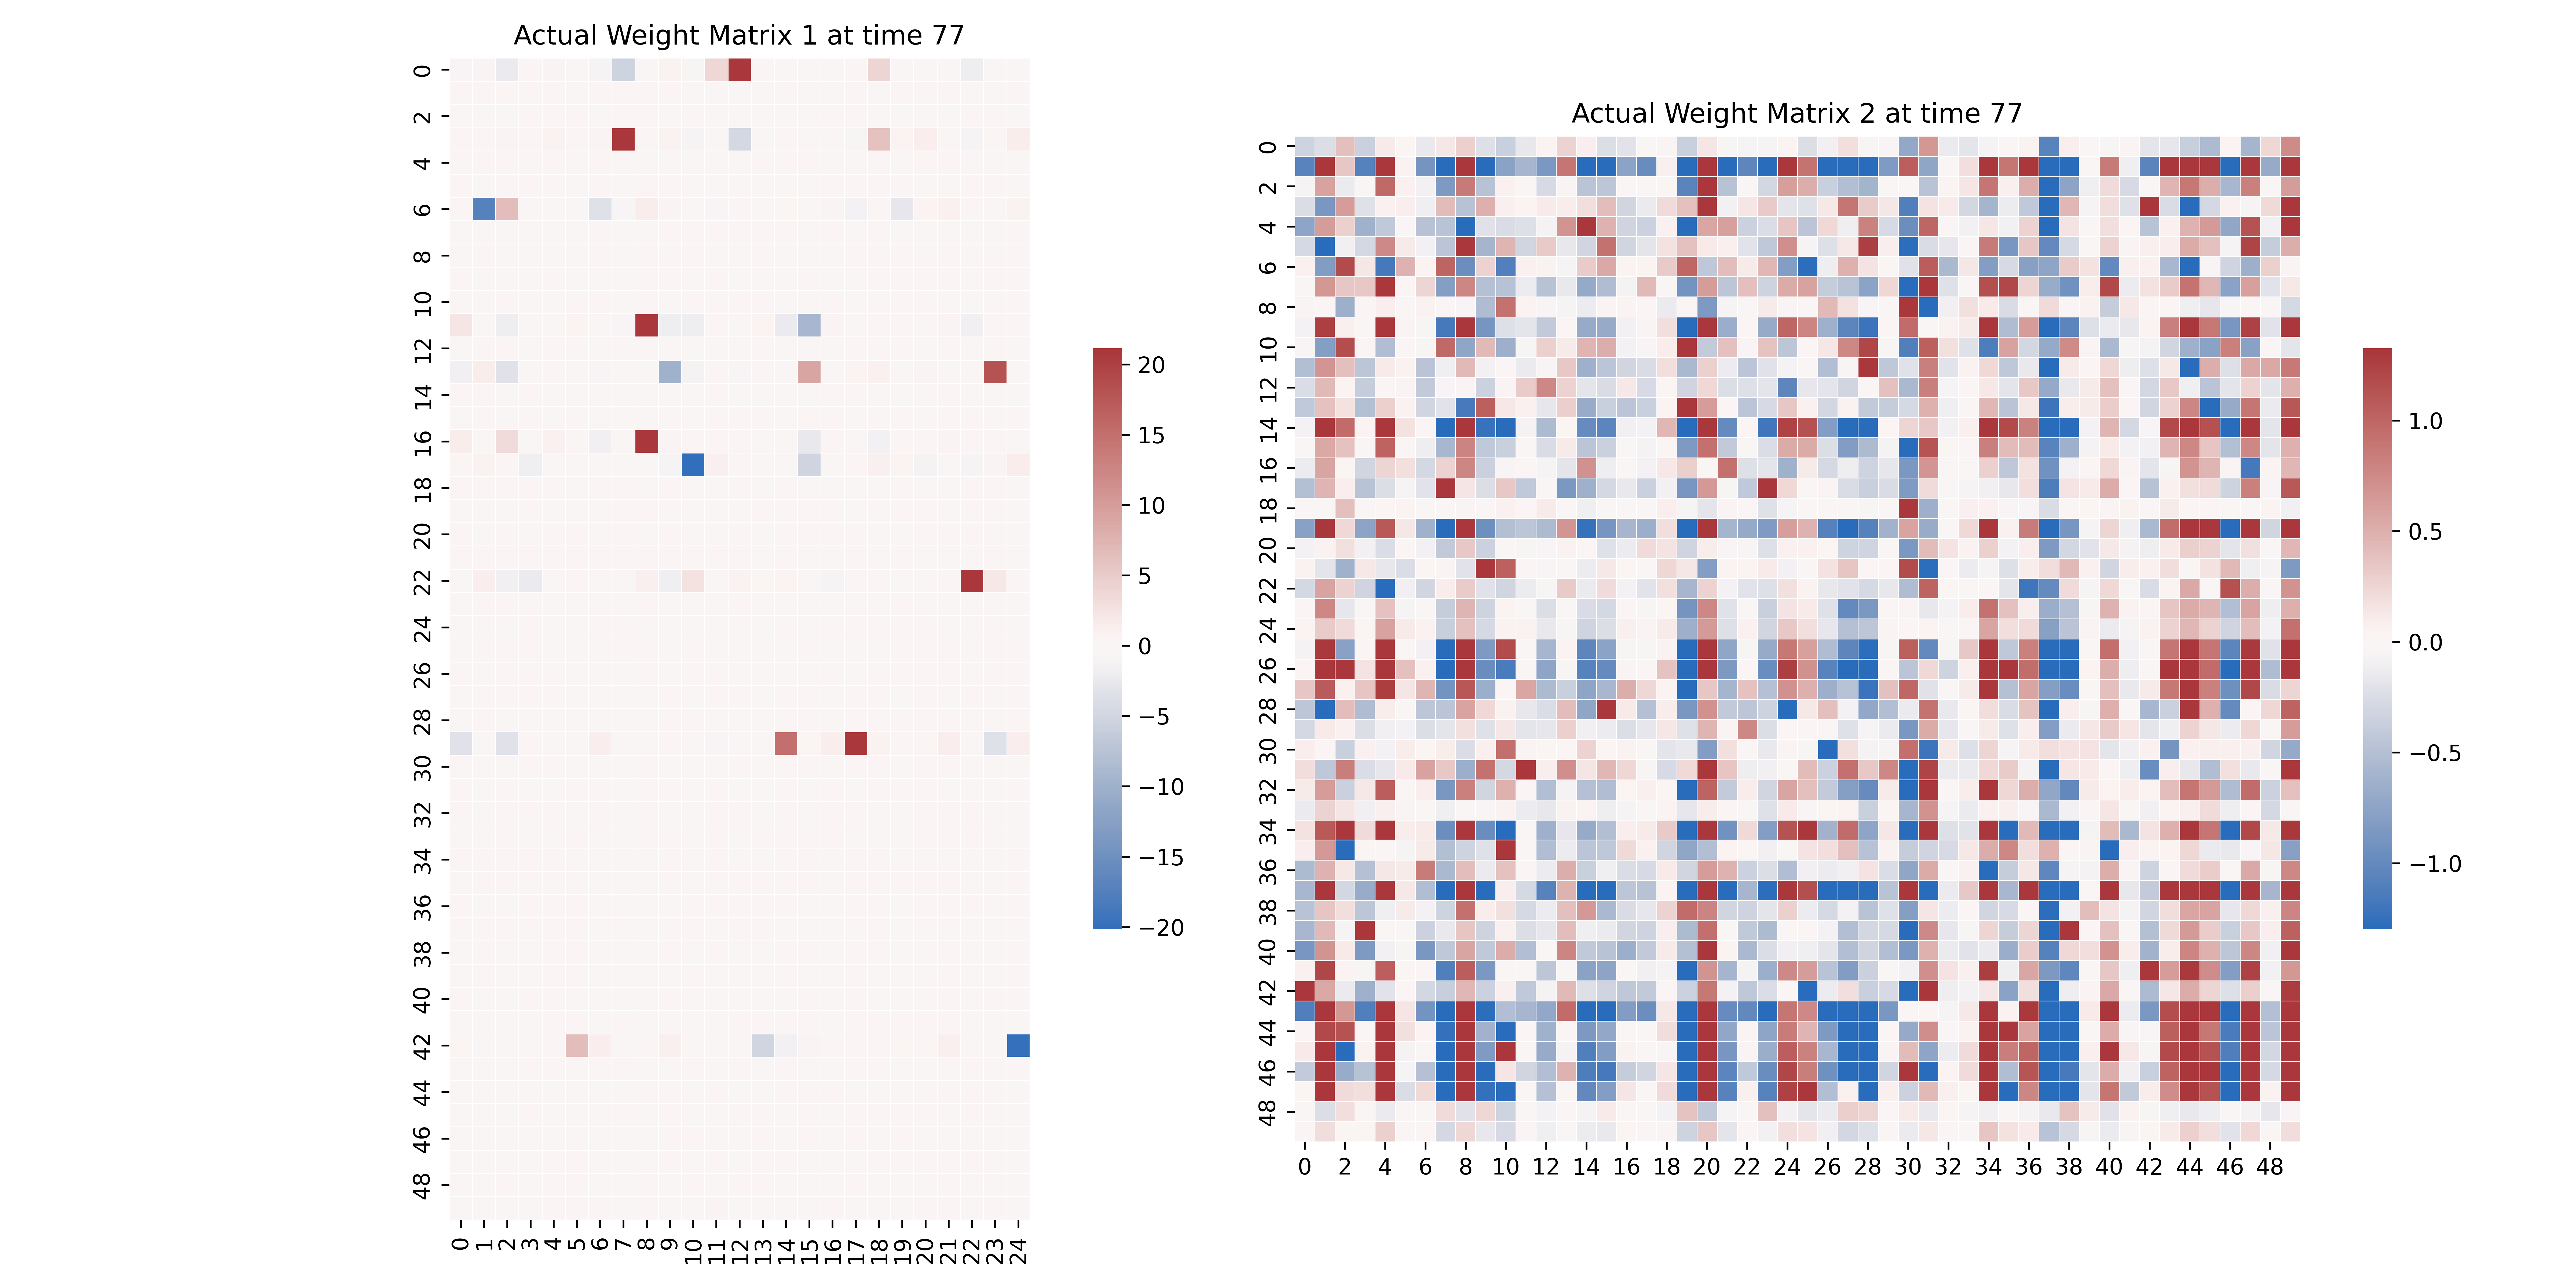
\includegraphics[width=\textwidth]{Actual_Weight_combined_77}
      \caption{T=77}
    \end{subfigure}
  \end{minipage}
  \caption{Actual weight}
\end{figure}

\begin{figure}[h!]
  \centering
  \begin{minipage}[b]{0.45\linewidth}
    \centering
    \begin{subfigure}[b]{\linewidth}
      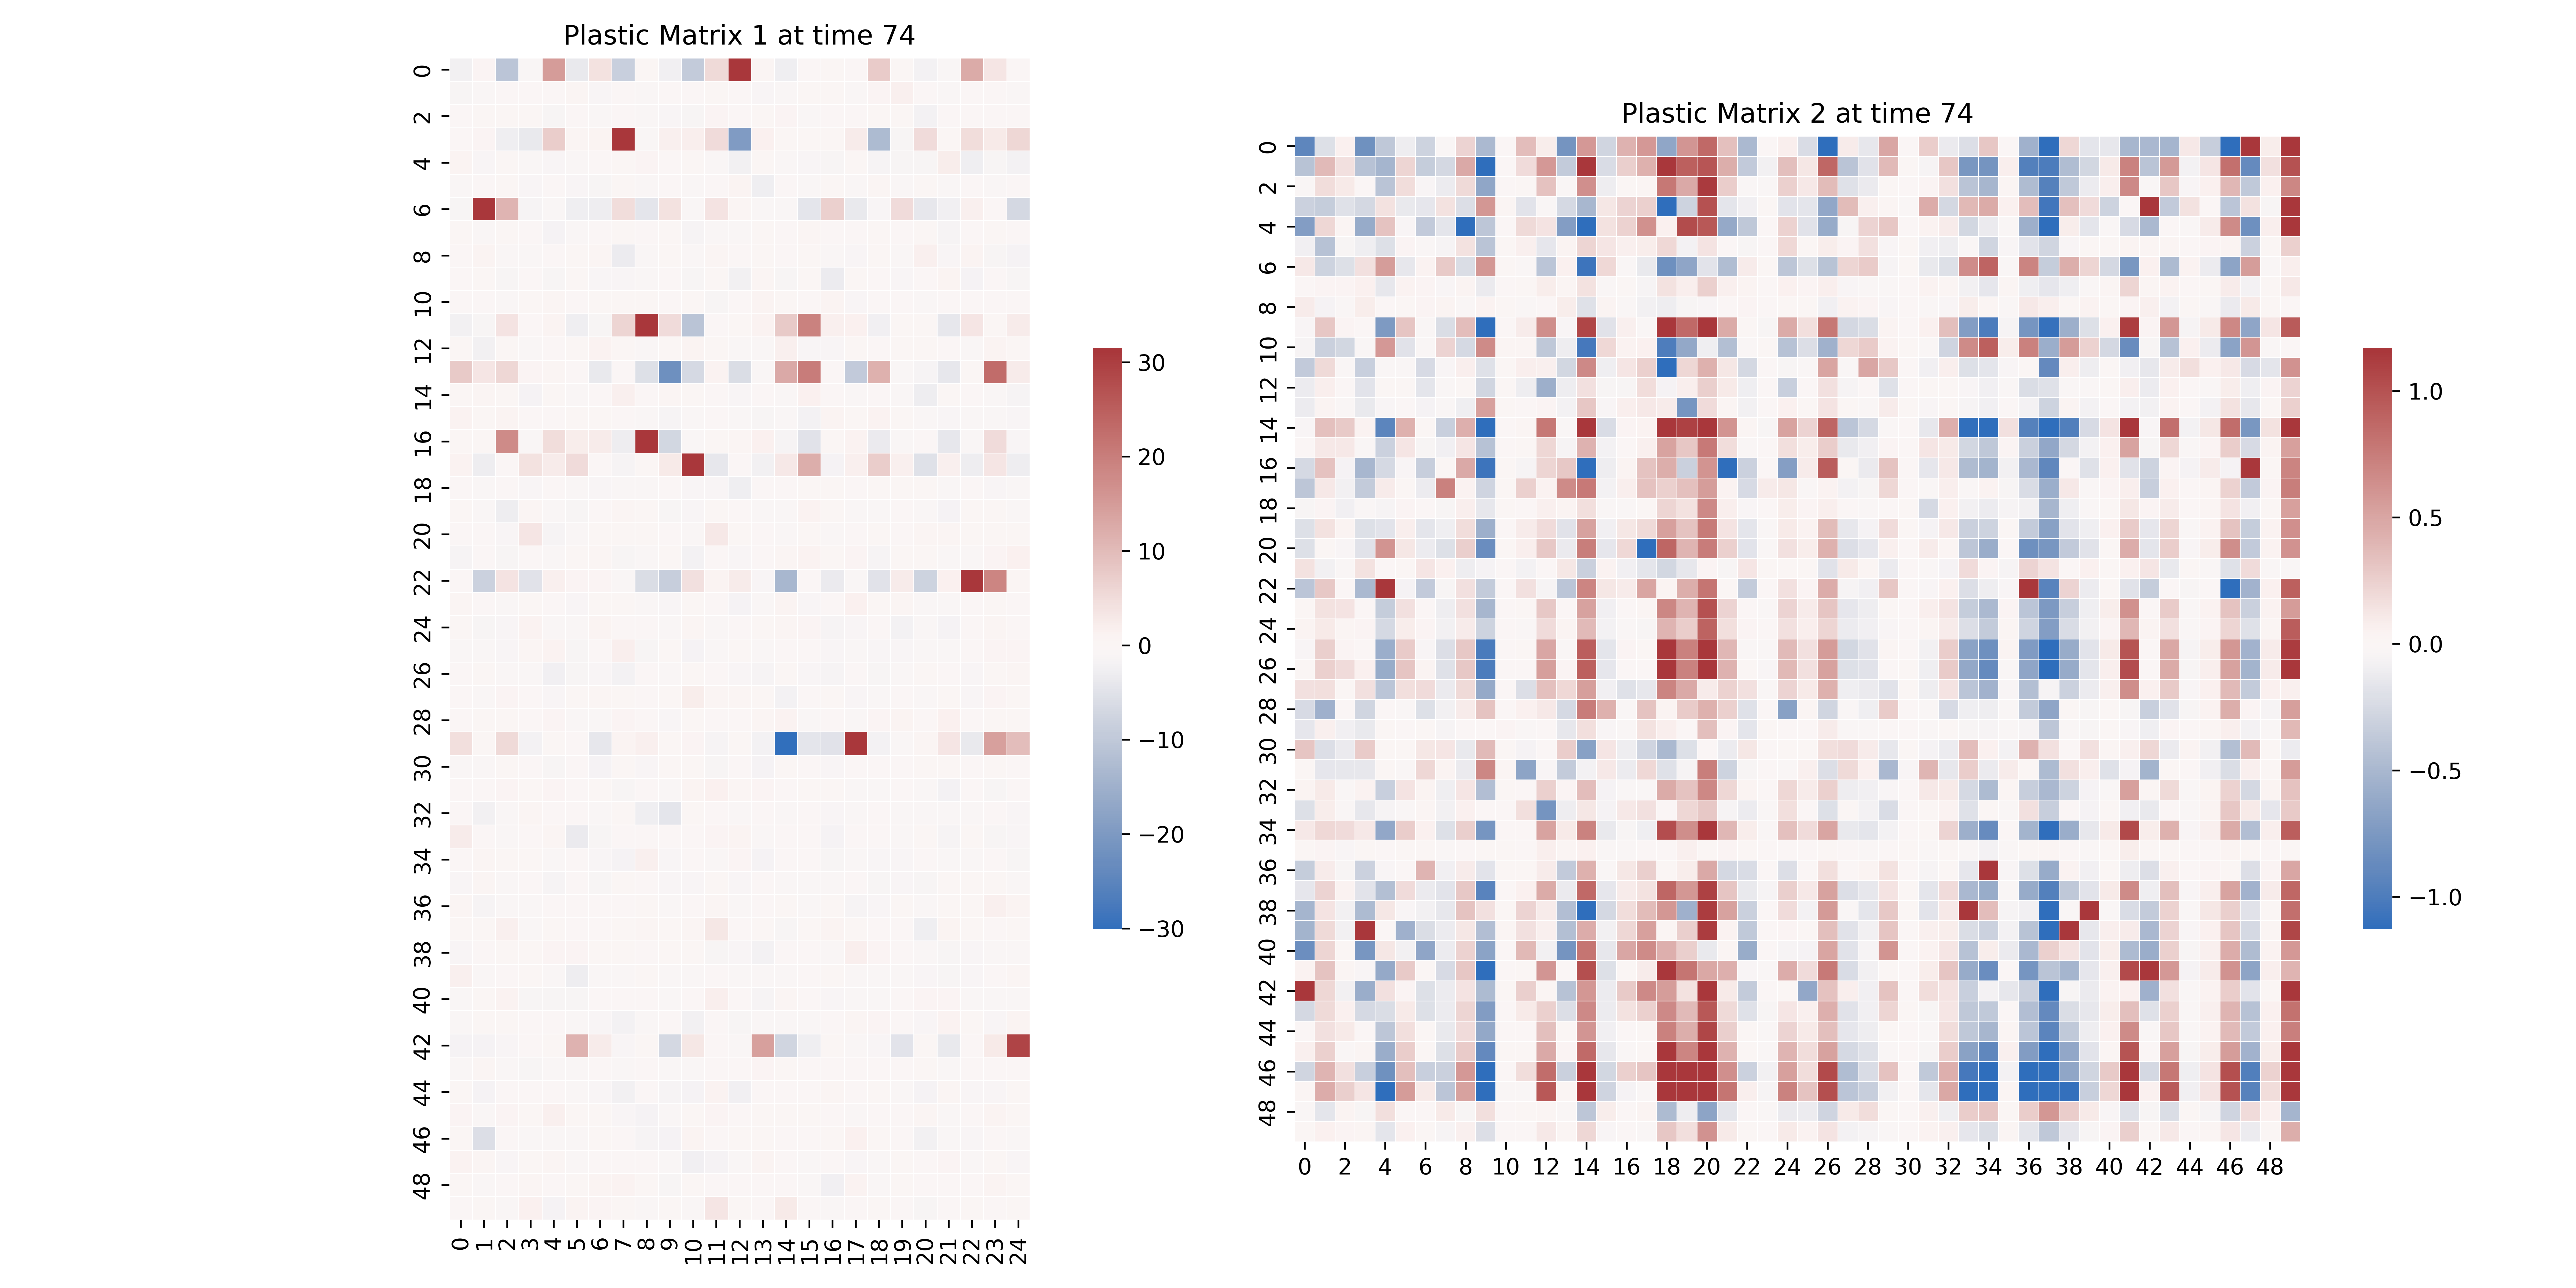
\includegraphics[width=\textwidth]{Plastic_combined_74}
      \caption{T=74}
    \end{subfigure}
    \vfill
    \begin{subfigure}[b]{\linewidth}
      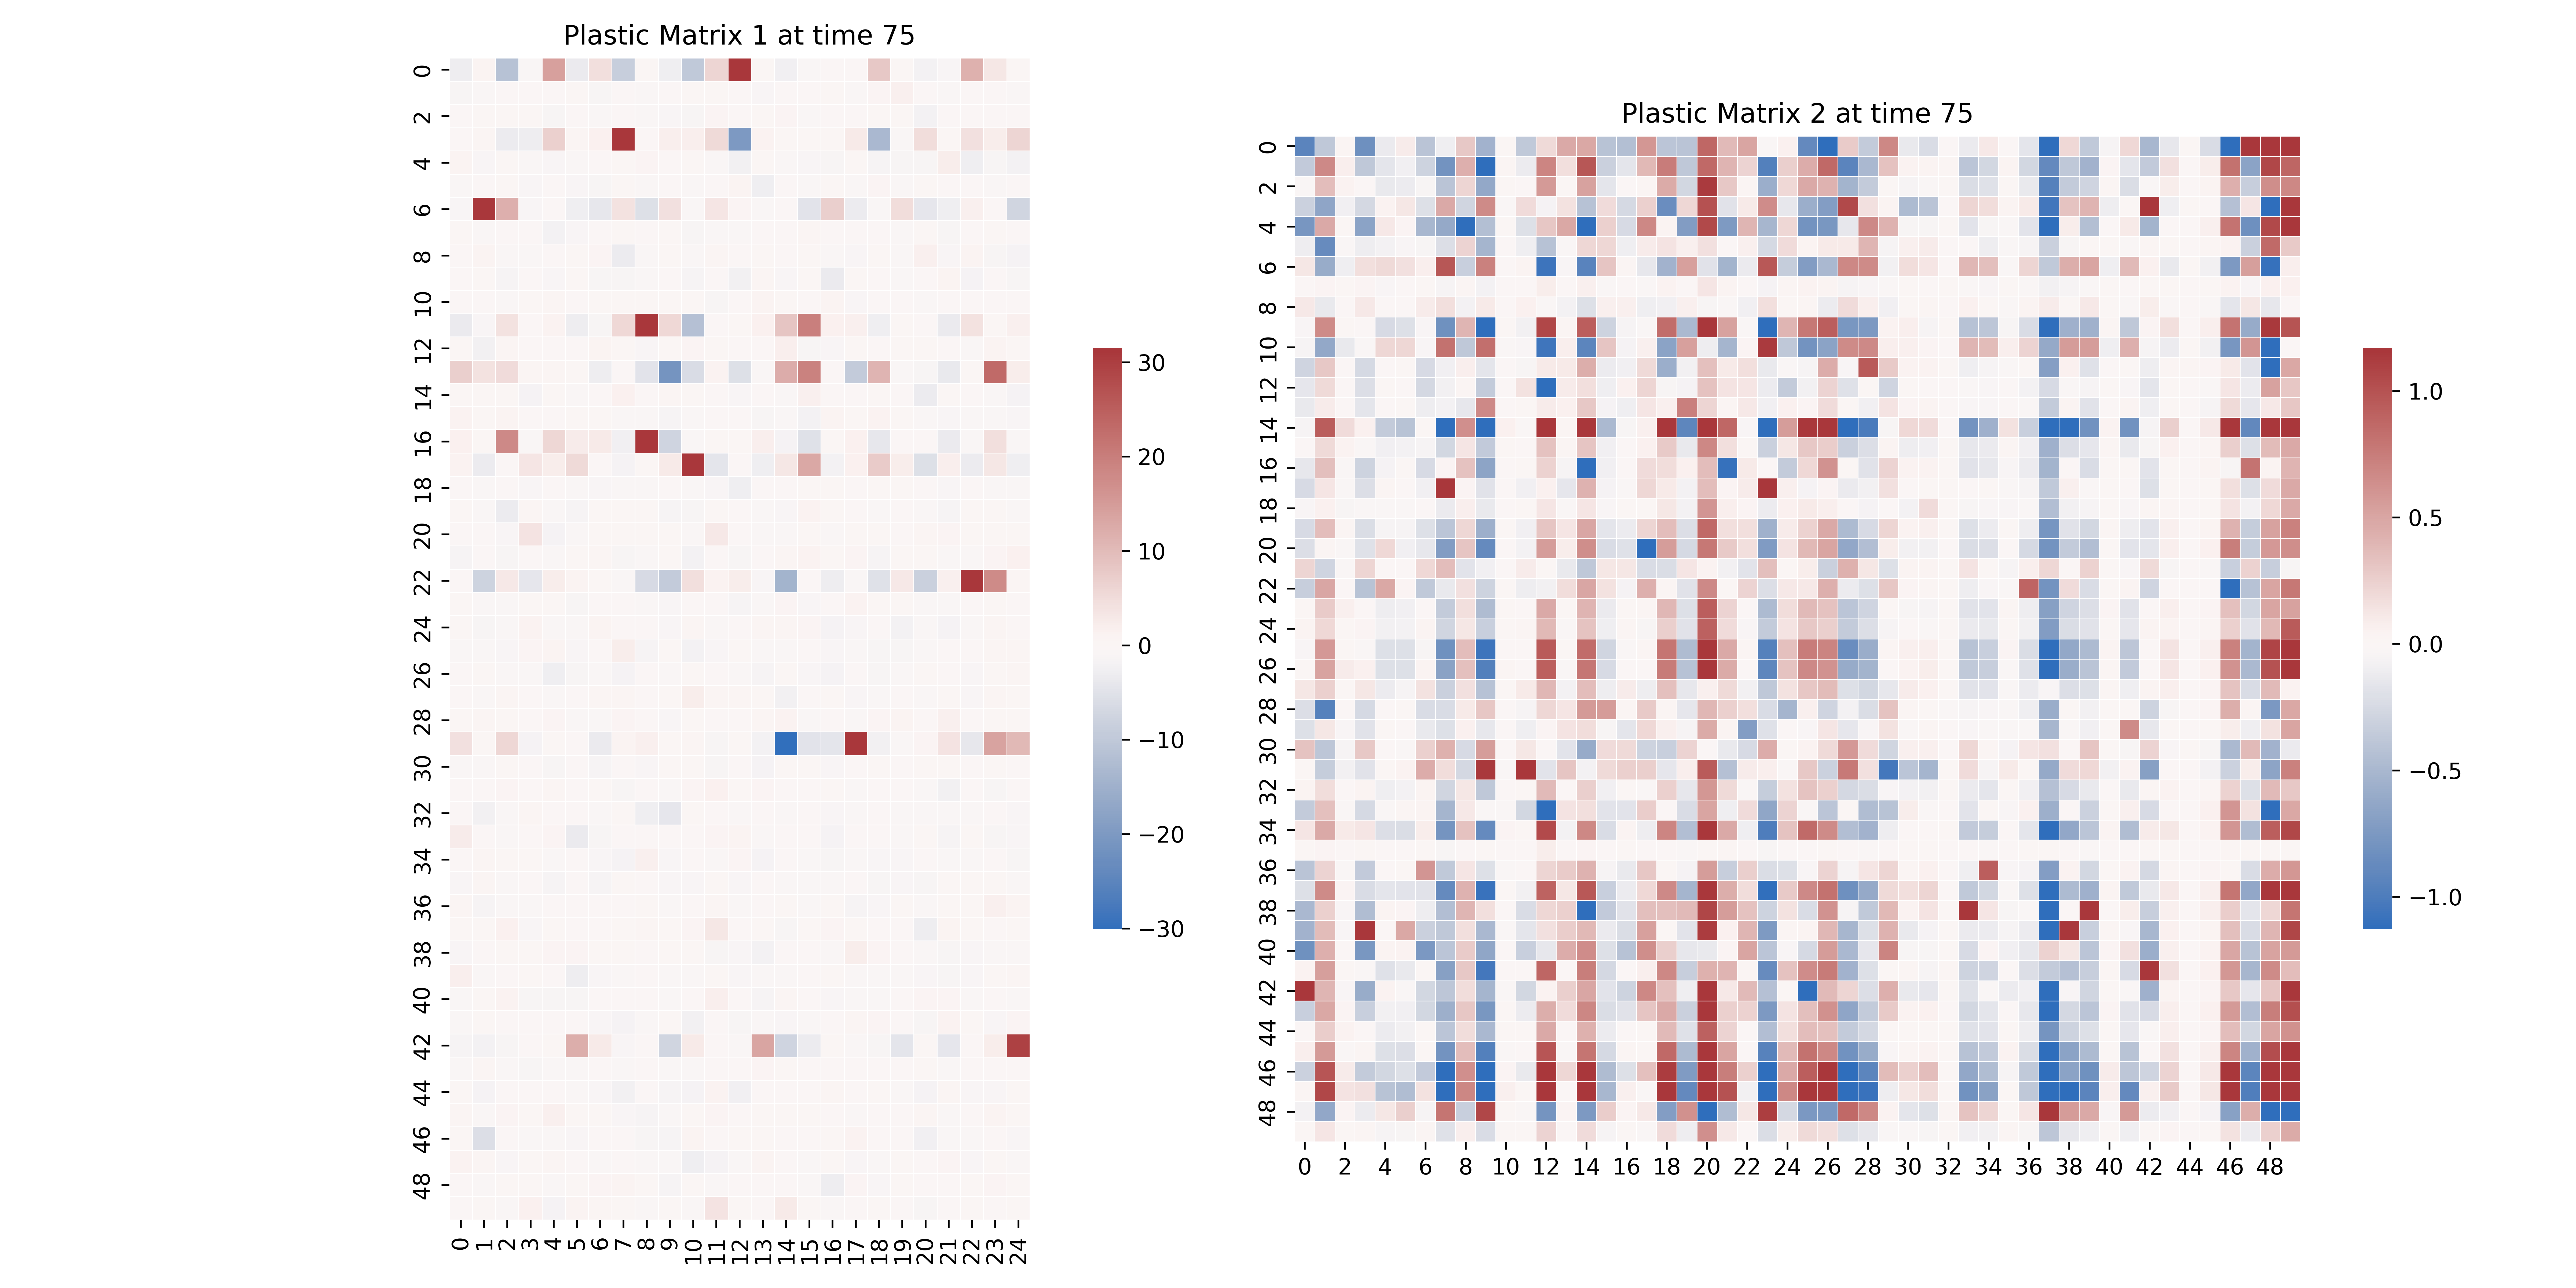
\includegraphics[width=\textwidth]{Plastic_combined_75}
      \caption{T=75}
    \end{subfigure}
  \end{minipage}
  \hfill
  \begin{minipage}[b]{0.45\linewidth}
    \centering
    \begin{subfigure}[b]{\linewidth}
      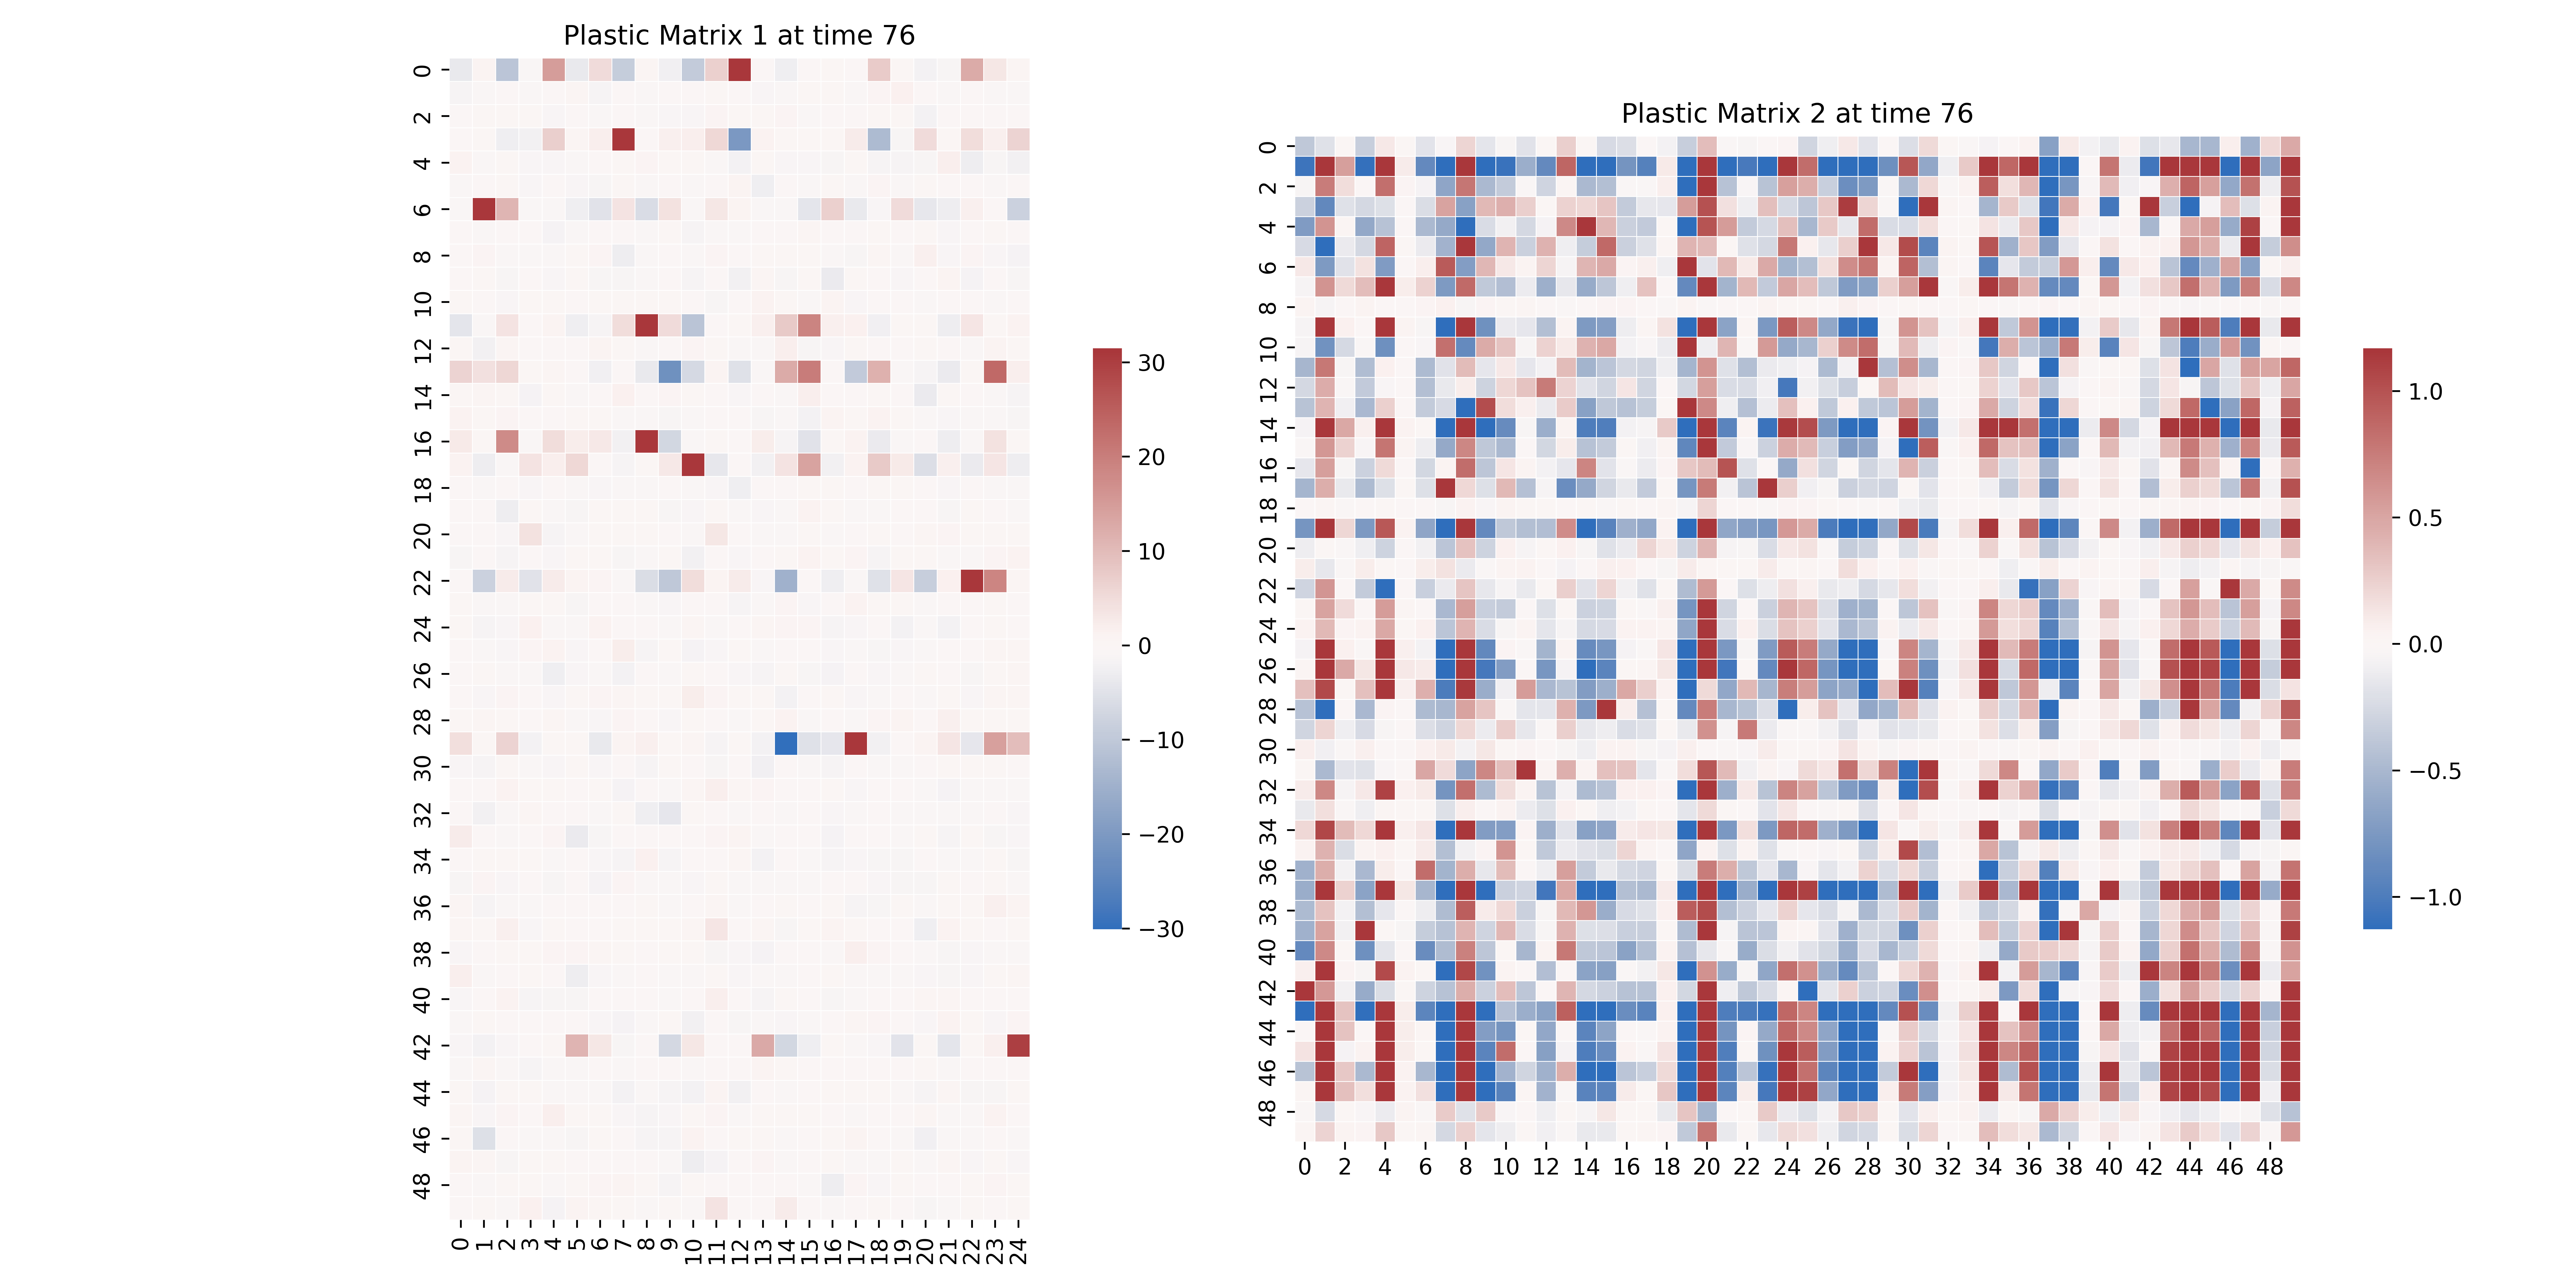
\includegraphics[width=\textwidth]{Plastic_combined_76}
      \caption{T=76}
    \end{subfigure}
    \vfill
    \begin{subfigure}[b]{\linewidth}
      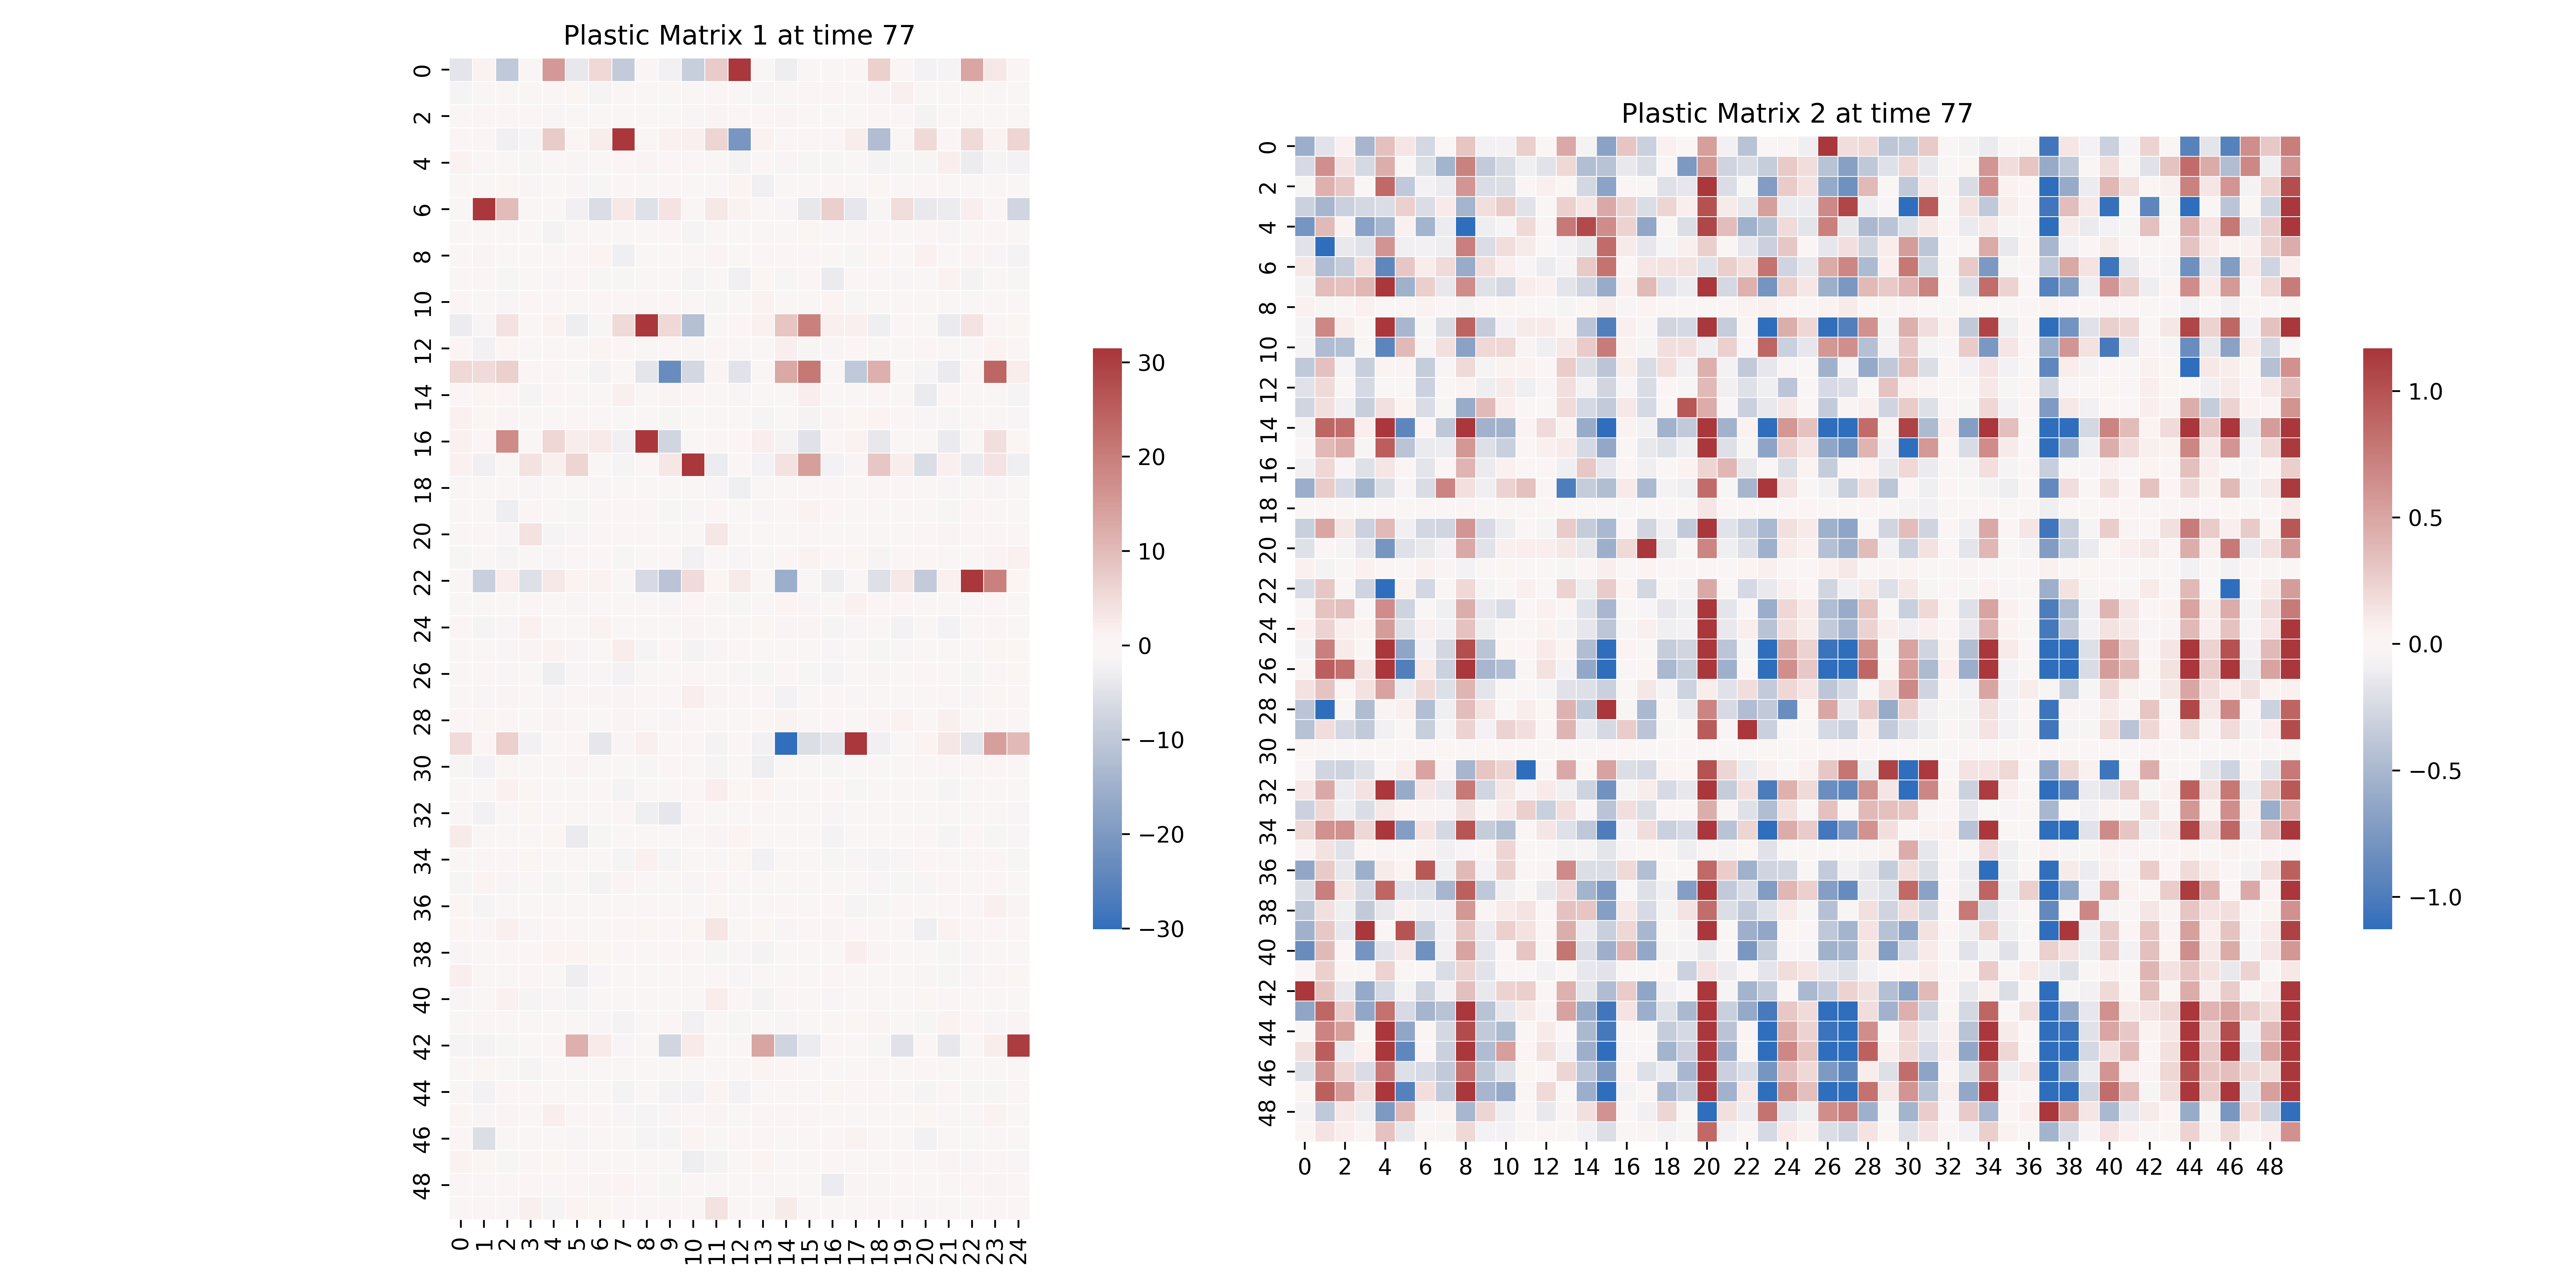
\includegraphics[width=\textwidth]{Plastic_combined_77}
      \caption{T=77}
    \end{subfigure}
  \end{minipage}
  \caption{Plasticity}
\end{figure}

Notice that the \textbf{M} is dominated by several elements and rarely changes. So a hypothesis would be that most of the identification work were done by the dynamic readout, whereas \textbf{M} merely serves as a memory source.


%Bibliography
\bibliographystyle{unsrt}  
\bibliography{references}  


\end{document}
